%=================================================================
% Predicting the Trainability of Hardware-Efficient Variational Quantum
% Circuits: A Data-Driven Model for Barren Plateaus
% Springer Nature journal template (sn-jnl), Math & Physical Sciences
% numbered reference style. Target: Quantum Machine Intelligence.
%
% Springer requires a SINGLE .tex file, so the result tables are inlined
% below. Every number and every table between the %%BEGIN/%%END markers is
% written by paper/qmi/fill_numbers.py from results/results.json, which is
% produced by  python -m qml_bp.analyze  -- do not edit those blocks by hand.
%=================================================================
\documentclass[pdflatex,sn-mathphys-num]{sn-jnl}

\usepackage{graphicx}
\usepackage{amsmath,amssymb,amsfonts}
\usepackage{booktabs}
\newsavebox{\tblbox}
% typeset a table at natural size, or scaled down to the text width if wider.
% Tables use the class's underlying float (tableorg) because its threeparttable
% wrapper does not accept a boxed tabular.
\newcommand{\fittable}[1]{\sbox{\tblbox}{#1}\ifdim\wd\tblbox>\textwidth
  \resizebox{\textwidth}{!}{\usebox{\tblbox}}\else\usebox{\tblbox}\fi}
\usepackage{multirow}

\theoremstyle{thmstyleone}
\newtheorem{theorem}{Theorem}

\newcommand{\Vbar}{\overline{\mathrm{Var}}}

%%BEGIN-NUMBERS
\newcommand{\Nrows}{20\,000}
\newcommand{\Nspecs}{20\,000}
\newcommand{\Nused}{19\,858}
\newcommand{\NallStruct}{142}
\newcommand{\Samples}{200}
\newcommand{\QubitLo}{2}
\newcommand{\QubitHi}{12}
\newcommand{\LayerLo}{1}
\newcommand{\LayerHi}{20}
\newcommand{\Narch}{5\,168}
\newcommand{\DesignSpace}{5\,280}
\newcommand{\MultMedian}{4}
\newcommand{\MultMax}{13}
\newcommand{\RowLeak}{95.0}
\newcommand{\BarrenFrac}{42.6}
\newcommand{\GlobalFrac}{50.4}
\newcommand{\LabelMean}{-1.88}
\newcommand{\LabelStd}{0.94}
\newcommand{\LabelMin}{-4.89}
\newcommand{\LabelMax}{-0.23}
\newcommand{\WithinVar}{0.013}
\newcommand{\TotalVar}{0.885}
\newcommand{\RsqCeiling}{0.985}
\newcommand{\RsqCeilingRy}{1.000}
\newcommand{\RsqCeilingPauli}{0.973}
\newcommand{\StructFracParams}{17.0}
\newcommand{\StructRowsAny}{87.0}
\newcommand{\LegacyFloorFrac}{9.6}
\newcommand{\LegacyCorr}{0.963}
\newcommand{\LegacyMAD}{0.16}
\newcommand{\LegacyFloorTrainable}{69}
\newcommand{\SpreadMedian}{0.6}
\newcommand{\SpreadPNineZero}{2.3}
\newcommand{\CostGap}{0.40}
\newcommand{\NFolds}{10}
\newcommand{\NFoldsK}{5}
\newcommand{\NRepeats}{2}
\newcommand{\RsqCV}{0.980}
\newcommand{\RsqCVsd}{0.003}
\newcommand{\MaeCV}{0.067}
\newcommand{\MaeCVsd}{0.003}
\newcommand{\AucCV}{0.998}
\newcommand{\AucCVsd}{0.000}
\newcommand{\AccCV}{0.979}
\newcommand{\AccCVsd}{0.004}
\newcommand{\RsqPhys}{0.682}
\newcommand{\RsqSub}{0.043}
\newcommand{\AucPhys}{0.927}
\newcommand{\GainOverPhys}{0.30}
\newcommand{\FracOfCeiling}{100}
\newcommand{\OofRsq}{0.980}
\newcommand{\OofRsqLo}{0.979}
\newcommand{\OofRsqHi}{0.982}
\newcommand{\RowRsq}{0.979}
\newcommand{\RowMae}{0.064}
\newcommand{\RowAuc}{0.999}
\newcommand{\ExtrapCut}{10}
\newcommand{\ExtrapTrainRows}{16\,278}
\newcommand{\ExtrapTestRows}{3\,580}
\newcommand{\RsqExtrap}{0.860}
\newcommand{\MaeExtrap}{0.320}
\newcommand{\RsqExtrapLo}{0.851}
\newcommand{\RsqExtrapHi}{0.869}
\newcommand{\MaeExtrapLo}{0.312}
\newcommand{\MaeExtrapHi}{0.327}
\newcommand{\RsqExtrapSeedSd}{0.001}
\newcommand{\AucExtrap}{0.995}
\newcommand{\RsqExtrapPhys}{0.326}
\newcommand{\MaeExtrapPhys}{0.665}
\newcommand{\RsqExtrapSub}{-1.027}
\newcommand{\RsqFull}{0.980}
\newcommand{\RsqPrim}{0.980}
\newcommand{\DeltaDerived}{0.000}
\newcommand{\AblTopOne}{qubit count $n$}
\newcommand{\AblTopOneDelta}{0.721}
\newcommand{\AblTopTwo}{cost locality}
\newcommand{\AblTopTwoDelta}{0.304}
\newcommand{\AblTopThree}{layers $L$}
\newcommand{\AblTopThreeDelta}{0.259}
\newcommand{\DeltaSize}{0.001}
\newcommand{\DeltaAddEff}{0.002}
\newcommand{\DeltaGatePrim}{0.155}
\newcommand{\DeltaAddCone}{0.001}
\newcommand{\DeltaAddBoth}{0.002}
\newcommand{\PythonVersion}{3.9.6}
\newcommand{\NumpyVersion}{2.0.2}
\newcommand{\SklearnVersion}{1.6.1}
\newcommand{\ValN}{200}
\newcommand{\ValState}{3.1e-16}
\newcommand{\ValGrad}{1.0e-15}
\newcommand{\ValGradN}{4\,792}
\newcommand{\ValStructN}{1153}
\newcommand{\ValStructViol}{0}
\newcommand{\RepeatN}{200}
\newcommand{\RepeatMAD}{0.021}
\newcommand{\RepeatMax}{0.20}
\newcommand{\RsqStruct}{0.969}
\newcommand{\RsqStructsd}{0.002}
\newcommand{\AucStruct}{0.997}
\newcommand{\StructNcoef}{124}
\newcommand{\RsqPhysEff}{0.750}
\newcommand{\GainOverStruct}{0.011}
\newcommand{\RsqExtrapStruct}{0.935}
\newcommand{\MaeExtrapStruct}{0.169}
\newcommand{\RsqExtrapMLPmean}{0.961}
\newcommand{\RsqExtrapMLPsd}{0.003}
\newcommand{\DeltaCostObs}{0.018}
\newcommand{\DeltaGateEff}{0.047}
\newcommand{\DeltaEffWeight}{0.000}
\newcommand{\GateGap}{0.08}
\newcommand{\NFeatures}{12}
\newcommand{\ConeExactRy}{90}
\newcommand{\ConeMadRy}{0.022}
\newcommand{\ConeMadPauli}{0.159}
\newcommand{\MaeENOneOnelocal}{0.185}
\newcommand{\MaeEPNOneOnelocal}{0.805}
\newcommand{\RsqENOneOnelocal}{0.951}
\newcommand{\RsqEPNOneOnelocal}{0.220}
\newcommand{\RsqEMNOneOnelocal}{0.971}
\newcommand{\MaeEMNOneOnelocal}{0.113}
\newcommand{\MaeENOneOneglobal}{0.280}
\newcommand{\MaeEPNOneOneglobal}{0.438}
\newcommand{\RsqENOneOneglobal}{0.811}
\newcommand{\RsqEPNOneOneglobal}{0.199}
\newcommand{\RsqEMNOneOneglobal}{0.911}
\newcommand{\MaeEMNOneOneglobal}{0.109}
\newcommand{\MaeENOneTwolocal}{0.309}
\newcommand{\MaeEPNOneTwolocal}{0.907}
\newcommand{\RsqENOneTwolocal}{0.876}
\newcommand{\RsqEPNOneTwolocal}{0.163}
\newcommand{\RsqEMNOneTwolocal}{0.956}
\newcommand{\MaeEMNOneTwolocal}{0.164}
\newcommand{\MaeENOneTwoglobal}{0.494}
\newcommand{\MaeEPNOneTwoglobal}{0.516}
\newcommand{\RsqENOneTwoglobal}{0.608}
\newcommand{\RsqEPNOneTwoglobal}{0.188}
\newcommand{\RsqEMNOneTwoglobal}{0.923}
\newcommand{\MaeEMNOneTwoglobal}{0.142}
\newcommand{\MaeENOneOne}{0.234}
\newcommand{\MaeEPNOneOne}{0.615}
\newcommand{\RsqENOneOne}{0.920}
\newcommand{\RsqEPNOneOne}{0.347}
\newcommand{\RsqEMNOneOne}{0.959}
\newcommand{\MaeEMNOneOne}{0.111}
\newcommand{\MaeENOneTwo}{0.400}
\newcommand{\MaeEPNOneTwo}{0.713}
\newcommand{\RsqENOneTwo}{0.815}
\newcommand{\RsqEPNOneTwo}{0.307}
\newcommand{\RsqEMNOneTwo}{0.953}
\newcommand{\MaeEMNOneTwo}{0.153}
\newcommand{\MaeELocal}{0.250}
\newcommand{\MaeEPLocal}{0.859}
\newcommand{\RsqELocal}{0.909}
\newcommand{\RsqEPLocal}{0.189}
\newcommand{\RsqEMLocal}{0.963}
\newcommand{\MaeEMLocal}{0.140}
\newcommand{\MaeEGlobal}{0.388}
\newcommand{\MaeEPGlobal}{0.477}
\newcommand{\RsqEGlobal}{0.695}
\newcommand{\RsqEPGlobal}{0.202}
\newcommand{\RsqEMGlobal}{0.919}
\newcommand{\MaeEMGlobal}{0.126}
\newcommand{\RsqExtrapMLPLo}{0.950}
\newcommand{\RsqExtrapMLPHi}{0.961}
\newcommand{\AucCutmOnepFive}{0.997}
\newcommand{\BarrenCutmOnepFive}{60}
\newcommand{\AucCutmTwopZero}{0.998}
\newcommand{\BarrenCutmTwopZero}{43}
\newcommand{\AucCutmTwopFive}{0.999}
\newcommand{\BarrenCutmTwopFive}{27}
\newcommand{\AucCutmThreepZero}{0.998}
\newcommand{\BarrenCutmThreepZero}{15}
\newcommand{\RsqCVMLP}{0.979}
\newcommand{\AucCVMLP}{0.999}
\newcommand{\RsqExtrapMLP}{0.956}
\newcommand{\RsqCVRandomForest}{0.976}
\newcommand{\AucCVRandomForest}{0.997}
\newcommand{\RsqExtrapRandomForest}{0.861}
\newcommand{\RsqCVExtraTrees}{0.978}
\newcommand{\AucCVExtraTrees}{0.998}
\newcommand{\RsqExtrapExtraTrees}{0.864}
\newcommand{\RsqCVkNN}{0.972}
\newcommand{\AucCVkNN}{0.995}
\newcommand{\RsqExtrapkNN}{0.864}
\newcommand{\RsqCVLinearbaseline}{0.891}
\newcommand{\AucCVLinearbaseline}{0.984}
\newcommand{\RsqExtrapLinearbaseline}{0.755}
\newcommand{\CrossLo}{seven}
\newcommand{\CrossHi}{eight}
\newcommand{\AllAboveMaxN}{4}
\newcommand{\BelowAtFive}{three}
\newcommand{\RowsAtFive}{1\,745}
\newcommand{\MinParamVar}{2.5\times10^{-9}}
\newcommand{\MinParamGradExp}{-4}
\newcommand{\TOFracMin}{94}
\newcommand{\TOFracMax}{99}
\newcommand{\TORhoMin}{0.08}
\newcommand{\TORhoMax}{0.19}
\newcommand{\TORhoTrueMin}{0.09}
\newcommand{\TORhoTrueMax}{0.19}
\newcommand{\TORhoPredMin}{0.08}
\newcommand{\TORhoPredMax}{0.17}
\newcommand{\TOCircuitsMin}{199}
\newcommand{\TOCircuitsMax}{299}
\newcommand{\ScreenSpearman}{0.989}
\newcommand{\ScreenTrainableFrac}{57.4}
\newcommand{\ScreenPrecFifty}{99.7}
\newcommand{\ScreenRecallFifty}{86.9}
\newcommand{\ScreenBottomTen}{100.0}
\newcommand{\ScreenTopPct}{20}
\newcommand{\ScreenTopK}{3\,971}
\newcommand{\GapHGBkSix}{-0.062}
\newcommand{\GapMLPkSix}{0.716}
\newcommand{\GapPhyskSix}{0.332}
\newcommand{\GapStructkSix}{0.839}
\newcommand{\GapMLPmeankSix}{0.631}
\newcommand{\GapMLPsdkSix}{0.110}
\newcommand{\GapMLPminkSix}{0.47}
\newcommand{\GapMLPmaxkSix}{0.81}
\newcommand{\GapHGBkSeven}{0.257}
\newcommand{\GapMLPkSeven}{0.832}
\newcommand{\GapPhyskSeven}{0.330}
\newcommand{\GapStructkSeven}{0.883}
\newcommand{\GapMLPmeankSeven}{0.846}
\newcommand{\GapMLPsdkSeven}{0.038}
\newcommand{\GapMLPminkSeven}{0.78}
\newcommand{\GapMLPmaxkSeven}{0.92}
\newcommand{\GapHGBkEight}{0.541}
\newcommand{\GapMLPkEight}{0.909}
\newcommand{\GapPhyskEight}{0.324}
\newcommand{\GapStructkEight}{0.902}
\newcommand{\GapMLPmeankEight}{0.906}
\newcommand{\GapMLPsdkEight}{0.017}
\newcommand{\GapMLPminkEight}{0.88}
\newcommand{\GapMLPmaxkEight}{0.93}
\newcommand{\GapHGBkNine}{0.729}
\newcommand{\GapMLPkNine}{0.946}
\newcommand{\GapPhyskNine}{0.324}
\newcommand{\GapStructkNine}{0.920}
\newcommand{\GapMLPmeankNine}{0.949}
\newcommand{\GapMLPsdkNine}{0.006}
\newcommand{\GapMLPminkNine}{0.94}
\newcommand{\GapMLPmaxkNine}{0.96}
\newcommand{\GapHGBkTen}{0.860}
\newcommand{\GapMLPkTen}{0.956}
\newcommand{\GapPhyskTen}{0.326}
\newcommand{\GapStructkTen}{0.935}
\newcommand{\GapMLPmeankTen}{0.961}
\newcommand{\GapMLPsdkTen}{0.003}
\newcommand{\GapMLPminkTen}{0.95}
\newcommand{\GapMLPmaxkTen}{0.96}
\newcommand{\ScreenByNPrec}{100}
\newcommand{\ScreenByNRecall}{35}
\newcommand{\ScrSpHGBmin}{0.94}
\newcommand{\ScrSpHGBmax}{0.98}
\newcommand{\ScrSpPhysmin}{0.58}
\newcommand{\ScrSpPhysmax}{0.64}
\newcommand{\ScrSpStructmin}{0.91}
\newcommand{\ScrSpStructmax}{0.97}
\newcommand{\ScrAboveTwelve}{26}
\newcommand{\ScrPrecTwelve}{99.5}
\newcommand{\LCHGBTwoFifty}{0.841}
\newcommand{\LCMLPTwoFifty}{0.877}
\newcommand{\LCHGBFiveHundred}{0.877}
\newcommand{\LCMLPFiveHundred}{0.929}
\newcommand{\LCHGBOneThousand}{0.914}
\newcommand{\LCMLPOneThousand}{0.943}
\newcommand{\LCHGBTwoThousand}{0.950}
\newcommand{\LCMLPTwoThousand}{0.962}
\newcommand{\LCHGBFourThousand}{0.969}
\newcommand{\LCMLPFourThousand}{0.970}
\newcommand{\LCHGBEightThousand}{0.977}
\newcommand{\LCMLPEightThousand}{0.978}
\newcommand{\LCHGBSixteenThousand}{0.980}
\newcommand{\LCMLPSixteenThousand}{0.979}
\newcommand{\LCRowsNinety}{1\,000}
\newcommand{\LCRowsSaturate}{4\,000}
\newcommand{\LargeN}{1\,991}
\newcommand{\LargeRsqMLPmean}{0.972}
\newcommand{\LargeRsqMLPsd}{0.002}
\newcommand{\LargeRsqHGB}{0.905}
\newcommand{\LargeMaeHGB}{0.316}
\newcommand{\LargeRsqHGBLo}{0.898}
\newcommand{\LargeRsqHGBHi}{0.913}
\newcommand{\LargeRsqHGBThirteen}{0.939}
\newcommand{\LargeRsqHGBFourteen}{0.876}
\newcommand{\LargeRsqMLP}{0.970}
\newcommand{\LargeMaeMLP}{0.137}
\newcommand{\LargeRsqMLPLo}{0.965}
\newcommand{\LargeRsqMLPHi}{0.974}
\newcommand{\LargeRsqMLPThirteen}{0.970}
\newcommand{\LargeRsqMLPFourteen}{0.969}
\newcommand{\LargeRsqPhys}{0.350}
\newcommand{\LargeMaePhys}{0.815}
\newcommand{\LargeRsqPhysLo}{0.326}
\newcommand{\LargeRsqPhysHi}{0.375}
\newcommand{\LargeRsqPhysThirteen}{0.354}
\newcommand{\LargeRsqPhysFourteen}{0.345}
\newcommand{\LargeRsqStruct}{0.951}
\newcommand{\LargeMaeStruct}{0.183}
\newcommand{\LargeRsqStructLo}{0.945}
\newcommand{\LargeRsqStructHi}{0.956}
\newcommand{\LargeRsqStructThirteen}{0.950}
\newcommand{\LargeRsqStructFourteen}{0.952}
\newcommand{\ClValN}{200}
\newcommand{\ClValParams}{15\,182}
\newcommand{\ClValMAD}{0.009}
\newcommand{\ClValMax}{0.12}
\newcommand{\ClValStruct}{2\,804}
\newcommand{\ClValStructHits}{0}
\newcommand{\ClValSamples}{65\,536}
\newcommand{\ClValSvSamples}{400}
\newcommand{\ClValBelow}{one}
\newcommand{\ClTrainRows}{7\,941}
\newcommand{\ClTestRows}{6\,000}
\newcommand{\ClResolved}{4\,370}
\newcommand{\ClCensored}{1\,630}
\newcommand{\ClStructCensOK}{66}
\newcommand{\ClStructRsqA}{0.92}
\newcommand{\ClStructMaeA}{0.22}
\newcommand{\ClMLPRsqA}{0.95 \pm 0.01}
\newcommand{\ClHGBRsqA}{0.71}
\newcommand{\ClResolvedFracA}{99}
\newcommand{\ClStructRsqB}{0.90}
\newcommand{\ClStructMaeB}{0.36}
\newcommand{\ClMLPRsqB}{0.89 \pm 0.04}
\newcommand{\ClHGBRsqB}{0.27}
\newcommand{\ClResolvedFracB}{96}
\newcommand{\ClStructRsqC}{0.80}
\newcommand{\ClStructMaeC}{0.54}
\newcommand{\ClMLPRsqC}{0.47 \pm 0.25}
\newcommand{\ClHGBRsqC}{0.31}
\newcommand{\ClResolvedFracC}{63}
\newcommand{\ClStructRsqD}{0.27}
\newcommand{\ClStructMaeD}{0.84}
\newcommand{\ClMLPRsqD}{-1.86 \pm 1.53}
\newcommand{\ClHGBRsqD}{0.47}
\newcommand{\ClResolvedFracD}{54}
\newcommand{\ClStructRsqE}{-0.07}
\newcommand{\ClStructMaeE}{0.99}
\newcommand{\ClMLPRsqE}{-5.11 \pm 3.48}
\newcommand{\ClHGBRsqE}{0.44}
\newcommand{\ClResolvedFracE}{52}
\newcommand{\ClLocStructA}{0.92}
\newcommand{\ClLocBiasA}{-0.14}
\newcommand{\ClGloStructA}{0.87}
\newcommand{\ClGloCensA}{0}
\newcommand{\ClLocStructB}{0.89}
\newcommand{\ClLocBiasB}{-0.23}
\newcommand{\ClGloStructB}{0.84}
\newcommand{\ClGloCensB}{5}
\newcommand{\ClLocStructC}{0.78}
\newcommand{\ClLocBiasC}{-0.40}
\newcommand{\ClGloStructC}{0.73}
\newcommand{\ClGloCensC}{35}
\newcommand{\ClLocStructD}{0.43}
\newcommand{\ClLocBiasD}{-0.66}
\newcommand{\ClGloStructD}{-0.35}
\newcommand{\ClGloCensD}{60}
\newcommand{\ClLocStructE}{0.23}
\newcommand{\ClLocBiasE}{-0.77}
\newcommand{\ClGloStructE}{-1.20}
\newcommand{\ClGloCensE}{98}
\newcommand{\ClShallowTrueA}{-2.07}
\newcommand{\ClShallowTrueE}{-2.03}
\newcommand{\ClShallowStructA}{-2.13}
\newcommand{\ClShallowStructE}{-2.52}
\newcommand{\ClFloorMinExp}{-7}
\newcommand{\ClFloorMaxExp}{-5}
\newcommand{\ClTrainGenerated}{8\,000}
\newcommand{\ClTrainUnresolved}{59}
\newcommand{\ClSlack}{0.3}
\newcommand{\ClLeTwentyResolved}{2\,045}
\newcommand{\ClLeTwentyTotal}{3\,611}
\newcommand{\ClLeTwentyStruct}{0.90}
\newcommand{\ClLeTwentyMLP}{0.85 \pm 0.07}
\newcommand{\ClLeTwentyHGB}{0.94}
\newcommand{\ClAbstractSentence}{With exact Clifford-sampled labels up to 32 qubits we measure a prediction horizon: an ensemble of neural networks stays on average within a factor of two of the true variance for five to six qubits beyond a training range of 12 or more qubits, for local costs. Prediction beyond that horizon is an open problem, for which we release a benchmark.}
\newcommand{\HzEnsemble}{ten}
\newcommand{\HzResGlobkEight}{100}
\newcommand{\HzResLockEight}{99}
\newcommand{\HzMLPkEight}{4}
\newcommand{\HzMLPIntkEight}{3--4}
\newcommand{\HzMLPWidekEight}{5}
\newcommand{\HzLocMLPkEight}{3}
\newcommand{\HzLocMLPIntkEight}{3--4}
\newcommand{\HzLocMLPWidekEight}{5}
\newcommand{\HzTablekEight}{5}
\newcommand{\HzTableIntkEight}{4--5}
\newcommand{\HzTableWidekEight}{8}
\newcommand{\HzLocTablekEight}{4}
\newcommand{\HzLocTableIntkEight}{4--4}
\newcommand{\HzLocTableWidekEight}{8}
\newcommand{\HzHGBkEight}{1}
\newcommand{\HzHGBIntkEight}{1--1}
\newcommand{\HzHGBWidekEight}{2}
\newcommand{\HzLocHGBkEight}{1}
\newcommand{\HzLocHGBIntkEight}{1--1}
\newcommand{\HzLocHGBWidekEight}{3}
\newcommand{\HzResGlobkTwelve}{99}
\newcommand{\HzResLockTwelve}{99}
\newcommand{\HzMLPkTwelve}{6}
\newcommand{\HzMLPIntkTwelve}{5--6}
\newcommand{\HzMLPWidekTwelve}{8}
\newcommand{\HzLocMLPkTwelve}{5}
\newcommand{\HzLocMLPIntkTwelve}{5--6}
\newcommand{\HzLocMLPWidekTwelve}{8}
\newcommand{\HzTablekTwelve}{4}
\newcommand{\HzTableIntkTwelve}{4--4}
\newcommand{\HzTableWidekTwelve}{10}
\newcommand{\HzLocTablekTwelve}{4}
\newcommand{\HzLocTableIntkTwelve}{3--5}
\newcommand{\HzLocTableWidekTwelve}{11}
\newcommand{\HzHGBkTwelve}{1}
\newcommand{\HzHGBIntkTwelve}{1--1}
\newcommand{\HzHGBWidekTwelve}{2}
\newcommand{\HzLocHGBkTwelve}{2}
\newcommand{\HzLocHGBIntkTwelve}{2--2}
\newcommand{\HzLocHGBWidekTwelve}{4}
\newcommand{\HzResGlobkSixteen}{81}
\newcommand{\HzResLockSixteen}{95}
\newcommand{\HzMLPkSixteen}{6}
\newcommand{\HzMLPIntkSixteen}{5--6}
\newcommand{\HzMLPWidekSixteen}{8}
\newcommand{\HzLocMLPkSixteen}{6}
\newcommand{\HzLocMLPIntkSixteen}{4--7}
\newcommand{\HzLocMLPWidekSixteen}{9}
\newcommand{\HzTablekSixteen}{3}
\newcommand{\HzTableIntkSixteen}{3--5}
\newcommand{\HzTableWidekSixteen}{10}
\newcommand{\HzLocTablekSixteen}{3}
\newcommand{\HzLocTableIntkSixteen}{2--5}
\newcommand{\HzLocTableWidekSixteen}{10}
\newcommand{\HzHGBkSixteen}{1}
\newcommand{\HzHGBIntkSixteen}{1--1}
\newcommand{\HzHGBWidekSixteen}{3}
\newcommand{\HzLocHGBkSixteen}{3}
\newcommand{\HzLocHGBIntkSixteen}{2--3}
\newcommand{\HzLocHGBWidekSixteen}{16}
\newcommand{\HzResGlobkTwenty}{36}
\newcommand{\HzResLockTwenty}{84}
\newcommand{\HzMLPkTwenty}{6}
\newcommand{\HzMLPIntkTwenty}{6--6}
\newcommand{\HzMLPWidekTwenty}{8}
\newcommand{\HzLocMLPkTwenty}{6}
\newcommand{\HzLocMLPIntkTwenty}{6--7}
\newcommand{\HzLocMLPWidekTwenty}{10}
\newcommand{\HzTablekTwenty}{3}
\newcommand{\HzTableIntkTwenty}{3--6}
\newcommand{\HzTableWidekTwenty}{12}
\newcommand{\HzLocTablekTwenty}{6}
\newcommand{\HzLocTableIntkTwenty}{3--8}
\newcommand{\HzLocTableWidekTwenty}{12}
\newcommand{\HzHGBkTwenty}{$\ge$12}
\newcommand{\HzHGBIntkTwenty}{1--12}
\newcommand{\HzHGBWidekTwenty}{12}
\newcommand{\HzLocHGBkTwenty}{$\ge$12}
\newcommand{\HzLocHGBIntkTwenty}{12--12}
\newcommand{\HzLocHGBWidekTwenty}{12}
\newcommand{\HzResGlobkTwentyfour}{24}
\newcommand{\HzResLockTwentyfour}{81}
\newcommand{\HzMLPkTwentyfour}{$\ge$8}
\newcommand{\HzMLPIntkTwentyfour}{7--8}
\newcommand{\HzMLPWidekTwentyfour}{8}
\newcommand{\HzLocMLPkTwentyfour}{$\ge$8}
\newcommand{\HzLocMLPIntkTwentyfour}{8--8}
\newcommand{\HzLocMLPWidekTwentyfour}{8}
\newcommand{\HzTablekTwentyfour}{$\ge$8}
\newcommand{\HzTableIntkTwentyfour}{3--8}
\newcommand{\HzTableWidekTwentyfour}{8}
\newcommand{\HzLocTablekTwentyfour}{$\ge$8}
\newcommand{\HzLocTableIntkTwentyfour}{8--8}
\newcommand{\HzLocTableWidekTwentyfour}{8}
\newcommand{\HzHGBkTwentyfour}{$\ge$8}
\newcommand{\HzHGBIntkTwentyfour}{8--8}
\newcommand{\HzHGBWidekTwentyfour}{8}
\newcommand{\HzLocHGBkTwentyfour}{$\ge$8}
\newcommand{\HzLocHGBIntkTwentyfour}{8--8}
\newcommand{\HzLocHGBWidekTwentyfour}{8}
\newcommand{\HzMaeTwelveDOne}{0.08}
\newcommand{\HzMaeTwelveDFour}{0.19}
\newcommand{\HzMaeTwelveDSix}{0.32}
\newcommand{\ClTargetHits}{2\,000}
\newcommand{\ClMaxSamples}{$2^{20}$}
\newcommand{\ClResolvedHits}{100}
\newcommand{\ClQmax}{32}
\newcommand{\TiedRows}{10\,000}
\newcommand{\TiedCeil}{0.989}
\newcommand{\TiedHGB}{0.983}
\newcommand{\TiedMLP}{0.981}
\newcommand{\TiedRule}{0.958}
\newcommand{\TiedPhys}{0.309}
\newcommand{\TiedExMLP}{0.969}
\newcommand{\TiedExHGB}{0.942}
\newcommand{\TiedExRule}{0.934}
\newcommand{\TiedTransfer}{-1.57}
\newcommand{\TiedOffset}{0.93}
\newcommand{\TiedCorr}{0.67}
\newcommand{\TiedBelowCut}{10}
\newcommand{\TiedLabelMin}{-3.25}
\newcommand{\TiedShortN}{100}
\newcommand{\TiedShortZero}{27}
\newcommand{\TiedShortOff}{27}
\newcommand{\GraphRows}{10\,000}
\newcommand{\GraphHGB}{0.975}
\newcommand{\GraphMLP}{0.974}
\newcommand{\GraphRule}{0.966}
\newcommand{\GraphDesignOnly}{0.936}
\newcommand{\GraphRuleCoef}{96}
\newcommand{\GraphExMLP}{0.923}
\newcommand{\GraphExHGB}{0.684}
\newcommand{\GraphExRule}{0.902}
\newcommand{\GraphConeMadRy}{0.002}
\newcommand{\GraphConeExactRy}{92}
\newcommand{\GraphNFeat}{19}
\newcommand{\TiedLargeN}{1\,000}
\newcommand{\TiedLargeMLP}{0.980 \pm 0.001}
\newcommand{\TiedLargeRule}{0.940}
\newcommand{\TiedLargeHGB}{0.960}
\newcommand{\TiedLargeBelowCut}{34}
\newcommand{\TiedLargeInRange}{91}
\newcommand{\TiedLargeLabelMin}{-3.74}
\newcommand{\TuneBest}{0.982}
\newcommand{\TuneSpread}{0.003}
\newcommand{\TuneGap}{0.013}
\newcommand{\TuneHeadroom}{0.003}
\newcommand{\TuneBestTied}{0.984}
\newcommand{\TuneGapTied}{0.026}
\newcommand{\LopoExtraRows}{9\,926}
\newcommand{\LopoDescRsq}{0.978}
\newcommand{\LopoIndexRsq}{0.978}
\newcommand{\LopoLinearUnseen}{0.946}
\newcommand{\LopoLinearSeen}{0.983}
\newcommand{\LopoLinearPhys}{0.692}
\newcommand{\LopoLinearUnseenMae}{0.128}
\newcommand{\LopoLinearUnseenAuc}{0.987}
\newcommand{\LopoLinearNoPhys}{0.732}
\newcommand{\LopoCircularUnseen}{0.950}
\newcommand{\LopoCircularSeen}{0.985}
\newcommand{\LopoCircularPhys}{0.824}
\newcommand{\LopoCircularUnseenMae}{0.132}
\newcommand{\LopoCircularUnseenAuc}{0.988}
\newcommand{\LopoCircularNoPhys}{0.694}
\newcommand{\LopoAllUnseen}{0.753}
\newcommand{\LopoAllSeen}{0.972}
\newcommand{\LopoAllPhys}{0.621}
\newcommand{\LopoAllUnseenMae}{0.241}
\newcommand{\LopoAllUnseenAuc}{0.972}
\newcommand{\LopoAllNoPhys}{0.414}
\newcommand{\LopoBrickUnseen}{0.930}
\newcommand{\LopoBrickSeen}{0.978}
\newcommand{\LopoBrickPhys}{0.669}
\newcommand{\LopoBrickUnseenMae}{0.141}
\newcommand{\LopoBrickUnseenAuc}{0.980}
\newcommand{\LopoBrickNoPhys}{0.925}
\newcommand{\LopoStarUnseen}{0.924}
\newcommand{\LopoStarSeen}{0.968}
\newcommand{\LopoStarPhys}{0.726}
\newcommand{\LopoStarUnseenMae}{0.156}
\newcommand{\LopoStarUnseenAuc}{0.996}
\newcommand{\LopoStarNoPhys}{0.742}
\newcommand{\LopoMinAuc}{0.97}
%%END-NUMBERS

\raggedbottom

\begin{document}

\title[Predicting the Trainability of Hardware-Efficient Variational Quantum Circuits]{Predicting
the Trainability of Hardware-Efficient Variational Quantum Circuits: A
Data-Driven Model for Barren Plateaus}

\author*[1]{\fnm{Md Habibur} \sur{Rahman}}\email{habib@gnu.ac.kr}

\affil*[1]{\orgdiv{Department of AI Convergence Engineering},
\orgname{Gyeongsang National University}, \orgaddress{\city{Jinju},
\country{Republic of Korea}}}

\abstract{Barren plateaus, the exponential decay of gradient variance with qubit
number, obstruct the training of variational quantum circuits. We study how well the gradient variance of hardware-efficient
circuits can be predicted from their architecture, and how far beyond the
training range such predictions can be trusted. We
simulate \Nrows{} circuits with 2 to 12 qubits; the label is the mean
gradient variance over all parameters whose gradient does not vanish
identically. Within the training range the label is predictable close to its noise ceiling: learners reach $R^2=\RsqCV$ on held-out
architectures against a ceiling of \RsqCeiling, a fitted linear table reaches
\RsqStruct{} and a five-coefficient textbook rule \RsqPhys, and the same
holds for layer-shared parameters and random entangling graphs. The last entangling layer changes the weight of the measured
observable; this effective weight and the causal cone, both
closed-form, let predictions transfer to unseen entanglement patterns. With exact Clifford-sampled
labels up to 32 qubits we define and measure a prediction horizon: for
local costs, an ensemble of neural networks stays on average within a
factor of two of the true variance for five to six qubits beyond a training
range of 12 or more qubits, and three beyond a range of 8. Beyond the horizon the error keeps growing,
and the models
underestimate how flat the flattest global-cost circuits are, which limits
their use for screening. Extending the horizon is posed as an open problem, with a benchmark. The predicted quantity is a finite-size proxy,
not optimization success or a proof of scaling.}

\keywords{Barren plateaus, Variational quantum circuits, Quantum machine
learning, Trainability, Gradient variance, Prediction horizon, Causal cone}

\maketitle

%=================================================================
\section{Introduction}\label{sec:intro}

Variational quantum algorithms (VQAs) are the leading way to use noisy
intermediate-scale quantum (NISQ) hardware~\cite{cerezo2021vqa}. A VQA works in
three steps. It encodes a problem into a parameterized quantum circuit, called
an ansatz. It then measures a cost function
$C(\theta)=\langle\psi(\theta)|O|\psi(\theta)\rangle$. Finally, a classical
optimizer updates the parameters $\theta$. This loop underlies variational
quantum eigensolvers, quantum approximate optimization, and most quantum
machine-learning (QML) classifiers~\cite{havlicek2019supervised,
farhi2018classification,schuld2020circuit}.

One problem stops this loop from scaling: the barren plateau
(BP)~\cite{mcclean2018barren,larocca2025barren}. On a barren plateau the
variance of the cost gradient, taken over random parameter settings, vanishes
exponentially in the number of qubits. The loss landscape becomes almost flat
almost everywhere, and gradient-based training stalls. Several causes are
known. Global cost observables trigger barren plateaus~\cite{cerezo2021cost}.
So do highly expressive or deep ans\"atze~\cite{holmes2022expressibility},
poor initialization~\cite{grant2019initialization}, and hardware
noise~\cite{wang2021noise}. Recent theory unifies many of these results
through the dynamical Lie algebra of the
circuit~\cite{ragone2024lie,fontana2024adjoint}. The common thread is that a
barren plateau is largely a property of the circuit design rather than of one
particular parameter setting.

The usual way to check a circuit is to measure it. One samples many random
parameter vectors, evaluates the gradients, and estimates their variance. This
is exactly the cost one wants to avoid when screening a large design space, and
it is hardest for many qubits, where barren plateaus matter most. This
motivates our question. Can a classical model predict the empirical gradient
variance of a variational circuit from its architecture alone, without
sampling any gradients?

We answer this question empirically for the hardware-efficient
ansatz~\cite{kandala2017hardware}, in three variants. We treat trainability
prediction as a supervised learning problem over circuit specifications. The
features are cheap architectural descriptors: small integers and categories.
The label is the gradient variance, computed once, offline, by exact
statevector simulation. Throughout, we use two standard machine-learning
scores. The coefficient of determination $R^2$ is the fraction of label
variance a regressor explains; $R^2=1$ is perfect and $R^2=0$ is no better than
predicting the mean. The area under the receiver operating characteristic
curve (AUC) is the probability that a classifier ranks a randomly chosen
positive example above a randomly chosen negative one; $0.5$ is chance and
$1$ is perfect. We also report the mean absolute error (MAE) of the
regressor, in $\log_{10}$ units.

Two methodological points shape the study. The first is the label. The
variance of the gradient with respect to a single parameter can vanish
identically for structural reasons, for example when the rotation commutes
with everything between it and the observable, and such a structural zero is
not a barren plateau. We therefore use the mean gradient variance over all
parameters, with structural zeros detected and excluded. The second is the
evaluation. The sampled design space contains far fewer distinct
architectures than the dataset has rows, so a row-wise random split places
identical feature vectors on both sides. All headline numbers come from
architecture-grouped cross-validation, and every learner is compared with
controls of increasing strength, from the training mean to a structured
linear model.

A word on terminology. We use \emph{trainability} in the operational sense
common in the barren-plateau literature: the magnitude of the gradient
variance. We do not claim to predict whether a particular optimizer, with a
particular budget, succeeds.

The contributions are as follows.
\begin{itemize}
\item A labeled dataset of \Nrows{} hardware-efficient circuits with exact
all-parameter gradient variances and structural zeros separated, with a
reproducible pipeline, and the finding that on unseen architectures the
label is predictable close to its noise ceiling ($R^2=\RsqCV$ against a ceiling of
\RsqCeiling) by flexible learners and, nearly as well, by a structured linear
model.
\item Two closed-form quantities, the weight of the observable after the
last entangling layer and the causal cone, which add little within the
training range but let predictions transfer out of it.
\item A measured prediction horizon. With exact Clifford-sampled labels up
to \ClQmax{} qubits, predictions for local-cost circuits stay on average within a factor of two
of the true variance for five to six qubits beyond a training range of 12
or more qubits (three beyond a range of 8); prediction beyond
it is posed as an open problem with a released benchmark.
\item Tests of generality: transfer to entanglement patterns absent from
training, and the same measurements on circuits with layer-shared
parameters, to which the Clifford shortcut does not apply, and on random
entangling graphs.
\end{itemize}

We also want to be clear about scope. We make no claim of quantum advantage.
The model is classical and the data is classically simulated. The predicted
quantity is an empirical, finite-size proxy for trainability within hardware-efficient layouts, not a proof of exponential scaling. The contribution is a data-driven
diagnostic for a known quantum-computing
bottleneck, in the spirit of recent calls for sober claims in quantum
machine
learning~\cite{schuld2022killoran,bowles2024benchmarking,cerezo2025simulability}.

%=================================================================
\section{Background and related work}\label{sec:background}

\subsection{Variational quantum circuits}
We use a hardware-efficient ansatz~\cite{kandala2017hardware}. Each layer
applies one single-qubit rotation to every qubit, then a fixed pattern of
two-qubit entangling gates. With $n$ qubits and $L$ layers the state is
\begin{equation}
|\psi(\theta)\rangle = \prod_{\ell=1}^{L}
  \Big[ U_{\mathrm{ent}} \prod_{q=1}^{n} R_{a_{\ell,q}}(\theta_{\ell,q}) \Big]
  |0\rangle^{\otimes n},
\label{eq:ansatz}
\end{equation}
where $R_a(\theta)=\exp(-i\theta\sigma_a/2)$ is a Pauli rotation about axis
$a\in\{x,y,z\}$ and $U_{\mathrm{ent}}$ is a layer of CZ or CX gates arranged
linearly, circularly, or all-to-all (Section~\ref{sec:spec} defines these
patterns precisely). The cost is the expectation of a Pauli-$Z$ string,
$C(\theta)=\langle\psi(\theta)|O|\psi(\theta)\rangle$, with either a local
observable $O=Z_0$ or a global one $O=Z_0Z_1\cdots Z_{n-1}$.

\subsection{Barren plateaus}
A circuit family has a barren plateau if
$\mathrm{Var}_\theta[\partial C/\partial\theta_k]$ decays exponentially in
$n$~\cite{mcclean2018barren}. This is a statement about a family of circuits
of growing size, not about any single circuit. Cerezo et
al.~\cite{cerezo2021cost} proved that global cost functions cause barren
plateaus even at shallow depth, whereas local costs can stay trainable up to
$O(\log n)$ depth. Cost locality is therefore a first-order design knob.
Expressibility~\cite{holmes2022expressibility} and entanglement also correlate
with flatter landscapes. Some structured architectures avoid the problem;
quantum convolutional networks are a proven
example~\cite{pesah2021absence}. The dimension of the dynamical Lie algebra
generated by the circuit gives a unified, exact characterization for many
families~\cite{ragone2024lie,fontana2024adjoint}, and a recent review
consolidates these results~\cite{larocca2025barren}.

Most of this work is analytical. It derives variance scaling laws for one
ansatz family at a time. Our work is empirical and complementary. We do not
prove a bound. Instead, we learn a predictive map across a heterogeneous but
finite space of architectures, at circuit sizes where the ground truth can be
simulated exactly.

\subsection{Exact gradients}\label{sec:gradients}
For gates generated by an operator with two eigenvalues, the parameter-shift
rule gives the exact gradient from two circuit
evaluations~\cite{mitarai2018circuit,schuld2019param}:
\begin{equation}
\frac{\partial C}{\partial\theta_k}
  = \tfrac{1}{2}\big[C(\theta + \tfrac{\pi}{2}e_k)
  - C(\theta - \tfrac{\pi}{2}e_k)\big].
\label{eq:pshift}
\end{equation}
Evaluating Eq.~\eqref{eq:pshift} for all $nL$ parameters costs $2nL$
simulations per parameter vector. On a classical simulator the same exact
gradient vector is available from a single backward pass. Reverse-mode
(adjoint) differentiation walks the circuit backwards once, maintaining the
state and the adjoint state, and yields every $\partial C/\partial\theta_k$ for
roughly the cost of three forward simulations. We use adjoint differentiation
for the dataset and verify it against Eq.~\eqref{eq:pshift}
(Section~\ref{sec:validation}). Each individual gradient is therefore exact
to floating-point precision. The label, a variance over finitely many
random parameter vectors, is nonetheless an estimator with its own sampling
uncertainty, which we quantify in Section~\ref{sec:label}.

\subsection{Related data-driven approaches}\label{sec:related}
Several lines of work use classical computation to rank or choose circuits
before training. Quantum architecture search (QAS) optimizes the circuit
structure itself, by differentiable relaxation~\cite{zhang2022dqas},
by sampling from a supernet~\cite{du2022qas}, or with training-free proxies
that score candidate circuits without optimizing
them~\cite{he2024tfqas}. Expressibility and entangling capability are
classical descriptors that are estimated by sampling and used to compare
ans\"atze~\cite{sim2019expressibility}. Lie-algebraic theory provides an
exact, closed-form trainability criterion for circuits whose generators are
known~\cite{ragone2024lie,fontana2024adjoint}.

Our work differs in three ways. The target is the empirical gradient variance
itself, not downstream task accuracy and not a proxy for it. The input is a
handful of architectural integers and categories, not a sampled statistic
such as expressibility, so a prediction costs microseconds. And the predictor
is learned across a heterogeneous design space and tested on architectures it
has never seen, including larger qubit counts. We are not aware of prior work
that casts barren-plateau severity as a directly predicted regression or
classification target from cheap architectural features and that also tests
extrapolation across qubit count. We regard the QAS proxies and the
Lie-algebraic criteria as complementary: a learned predictor of the kind
studied here could serve as a zero-cost filter inside a QAS loop.

\paragraph{Efficient computation of gradient variance.} For some circuit
families the gradient variance can be bounded or computed without
simulating a $2^n$-dimensional state. Uvarov and
Biamonte~\cite{uvarov2021locality} bound it through the causal cone of each
Pauli term of the cost. Napp~\cite{napp2022quantifying} relates the landscape
flatness of unstructured ans\"atze to a random walk and estimates it by
Monte Carlo. Letcher et al.~\cite{letcher2024tight} derive tight and
efficiently computable gradient bounds for a large class of circuits without
design assumptions. The circuits studied here admit a particularly simple
exact method. Every angle appears once with a Pauli generator, so the cost is
a trigonometric polynomial of degree one in each angle, the squared gradient
has degree two, and its uniform average equals its average over the four
angles $\{0,\pi/2,\pi,3\pi/2\}$. At those angles every gate is Clifford and
the observable can be propagated as a single Pauli string at any $n$. We use
this in Section~\ref{sec:clifford} to label circuits far beyond statevector
reach. It also bears on the motivation for a learned predictor, which we
discuss in Section~\ref{sec:discussion}.

%=================================================================
\section{Methods}\label{sec:methods}
Figure~\ref{fig:pipeline} summarizes the pipeline from a sampled circuit
specification to a predicted trainability value.

\begin{figure}[t]
\centering
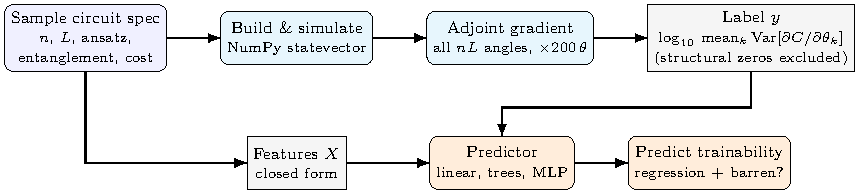
\includegraphics[width=\textwidth]{figs/pipeline.pdf}
\caption{Method pipeline. A random circuit specification is built and
simulated exactly with our NumPy statevector simulator. The exact gradient
with respect to every rotation angle is obtained by adjoint differentiation
for \Samples{} random parameter vectors. The label $y$ is $\log_{10}$ of the
mean gradient variance over all parameters that are not structural zeros.
Closed-form architectural features $X$ are read directly from the
specification, and predictors ranging from a structured linear model to
gradient-boosted trees and a neural network are trained on $(X,y)$.}
\label{fig:pipeline}
\end{figure}

\subsection{Circuit specification and feature space}\label{sec:spec}
Each datapoint is a specification, or spec. A spec fixes one parameterized circuit
through six design parameters: the qubit count $n$, the layer count $L$, the
rotation scheme, the entanglement pattern, the entangler gate, and the cost
observable. Table~\ref{tab:features} lists the twelve-element feature vector we
hand to the model. Six entries are the design parameters themselves, which we
call the primitive features. Six are derived from them in closed form; two
of these, the effective observable weight and the causal cone, encode
physics that the primitive features carry only implicitly. No quantum simulation
is needed to obtain any feature.


\begin{tableorg}[t]
\centering\tablebodyfont
\caption{Architectural features. The first six are the design parameters,
each drawn independently and uniformly from the listed values; the last six
are deterministic functions of them.}
\label{tab:features}
\fittable{%
\begin{tabular}{@{}llll@{}}
\toprule
\textbf{Feature} & \textbf{Meaning} & \textbf{Sampled values} & \textbf{Type}\\
\midrule
\texttt{n\_qubits}         & number of qubits $n$ & 2--12 & primitive\\
\texttt{n\_layers}         & number of ansatz layers $L$ & 1--20 & primitive\\
\texttt{ansatz\_type}      & rotation scheme & fixed-\texttt{ry}, random-Pauli & primitive\\
\texttt{entangle\_pattern} & entanglement pattern & linear, circular, all-to-all & primitive\\
\texttt{entangler\_gate}   & entangler gate & CZ, CX & primitive\\
\texttt{cost\_global}      & cost observable & local $Z_0$, global $Z^{\otimes n}$ & primitive\\
\texttt{n\_params}         & $nL$ trainable rotations & & derived\\
\texttt{n\_entanglers}     & entangling gates per layer $\times L$ & & derived\\
\texttt{depth\_ratio}      & $L/n$, ansatz layers per qubit & & derived\\
\texttt{cost\_weight\_eff} & weight of the observable after the last entangling layer & & derived\\
\texttt{cone\_qubits}      & qubits in the backward causal cone of the observable & & derived\\
\texttt{cone\_frac}        & fraction of rotations inside the causal cone & & derived\\
\botrule
\end{tabular}%
}
\end{tableorg}

\paragraph{Rotation scheme.} With the fixed-\texttt{ry} scheme every rotation
in Eq.~\eqref{eq:ansatz} is $R_y$. With the random-Pauli scheme the axis
$a_{\ell,q}$ of each of the $nL$ rotations is drawn independently and
uniformly from $\{x,y,z\}$ once, when the spec is created, from the spec's
own random seed. The axis pattern is then fixed for that spec: it does not
change between the random parameter vectors used to label the circuit. Two
random-Pauli specs with the same feature vector can therefore have different
axis patterns. The feature vector does not encode the pattern, so this
variation acts as label noise from the model's point of view. We quantify its
effect in Section~\ref{sec:data}.

\paragraph{Entanglement pattern.} Each layer applies the entangler gate to a
fixed list of ordered qubit pairs $(a,b)$, in list order, after the rotation
layer. The linear pattern uses the $n-1$ nearest-neighbor pairs
$(0,1),(1,2),\dots,(n-2,n-1)$. The circular pattern adds the wrap-around pair
$(n-1,0)$, giving $n$ gates per layer. The all-to-all pattern uses every pair
$(a,b)$ with $a<b$, giving $n(n-1)/2$ gates per layer. For CX the first
qubit of each pair is the control and the second is the target; CZ is
symmetric. The same list is used in every layer.

\paragraph{Cost observable and its effective weight.} The local cost
measures $Z$ on qubit $0$ only. The global cost measures the parity operator
$Z^{\otimes n}$. These are the nominal observables. The last entangling
layer sits between the final rotations and the measurement, and it is a
Clifford circuit, so it can be absorbed into the observable:
$C=\langle\psi'|O_{\mathrm{eff}}|\psi'\rangle$ with
$O_{\mathrm{eff}}=U_{\mathrm{ent}}^\dagger O\,U_{\mathrm{ent}}$ and
$|\psi'\rangle$ the state after the final rotations. CZ is diagonal and
leaves a $Z$-string unchanged. CX maps $Z$ on its target to $Z$ on control
and target, so a layer of CX gates maps the nominal $Z$-string to a
different $Z$-string. We call the number of qubits on which
$O_{\mathrm{eff}}$ acts the effective weight. It follows from the design
parameters in closed form and can differ sharply from the nominal weight:
with circular CX entanglement the nominally local cost has effective weight
$n-1$, and with all-to-all CX entanglement the nominally global cost has
effective weight
$1$ (Table~\ref{tab:effweight}). The effect follows from the convention,
common for hardware-efficient ans\"atze and used here, that every layer
ends with its entangling gates, so that an entangling layer directly
precedes the measurement. An ansatz that ends with a rotation layer has
effective weight equal to nominal weight. The practical point is that a
layout convention can silently change the locality of the cost.

\paragraph{Causal cone.} A rotation can only affect the cost if some
sequence of entangling gates connects it to the support of the observable.
Propagating the observable backward through the circuit, and keeping for
every qubit the set of Pauli types it can carry (a per-qubit relaxation that
drops correlations between qubits and therefore gives an outer bound), yields
two closed-form quantities: the number of qubits that can carry a
non-identity Pauli when the observable reaches the input, which we call
\texttt{cone\_qubits}, and the fraction of rotations at which the incoming
Pauli can anticommute with the rotation generator, \texttt{cone\_frac}. For
the fixed-\texttt{ry} scheme the rotation axes are known and the bound is
tight: \texttt{cone\_frac} equals the exact non-structural fraction of
parameters in \ConeExactRy\% of circuits, with mean absolute difference
\ConeMadRy. For random-Pauli circuits the axes are hidden and the generic
case is assumed (mean absolute difference \ConeMadPauli). The causal cone
matters for extrapolation: for a local observable and a shallow circuit the
cone is smaller than the circuit, and once it is, adding qubits adds only
parameters with zero gradient. Uvarov and Biamonte~\cite{uvarov2021locality}
bound the gradient variance through the same quantity.

\subsection{Label generation}\label{sec:label}
We label each spec in four steps. First, we draw \Samples{} parameter vectors
$\theta\sim\mathrm{Unif}[0,2\pi)^{nL}$. Second, for each $\theta$ we compute
the exact gradient vector $\nabla_\theta C$ by adjoint differentiation. Third,
for every parameter $k$ we compute the population variance $v_k$ of
$\partial C/\partial\theta_k$ over the \Samples{} samples. Fourth, we detect
structural zeros and average the remaining variances.

\paragraph{Structural zeros.} Some rotations have a gradient that is
identically zero for every $\theta$. This happens when the rotation commutes
with everything between it and the observable: for example an $R_z$ applied
immediately before a $Z$ measurement on the same qubit, a rotation on a
qubit outside the light cone of a local observable in a shallow circuit, or a
rotation on the control qubit of CX gates that lead only to the observable's
support. Such a parameter is untrainable, but the reason is an exact
symmetry, not a barren plateau. We flag parameter $k$ as a structural zero
when $\max_\theta|\partial C/\partial\theta_k|<10^{-10}$ over all \Samples{}
samples. Section~\ref{sec:validation} verifies that flagged parameters remain
exactly zero on fresh samples, so the flag is a property of the circuit and
not of the sample. The smallest per-parameter variance among non-flagged parameters in the
dataset is $\MinParamVar$, which corresponds to gradient components of order
$10^{\MinParamGradExp}$, more than five orders of magnitude above the
tolerance, so the two populations do not overlap.

\paragraph{Regression and classification labels.} Let $\mathcal{K}$ be the
set of parameters that are not structural zeros. The label is
\begin{equation}
y=\log_{10}\Vbar,\qquad
\Vbar=\frac{1}{|\mathcal{K}|}\sum_{k\in\mathcal{K}} v_k .
\label{eq:label}
\end{equation}
No floor or clipping is applied; $\Vbar$ is strictly positive by
construction, and the smallest value in the dataset is
$10^{\LabelMin}$. Specs with $\mathcal{K}=\emptyset$ (every parameter a
structural zero) cannot be labeled and are excluded; there are \NallStruct{}
such rows. The classification label is $\mathbb{1}[y<-2]$, which we call
``barren'' for brevity. The cutoff is a modeling choice: $\Vbar<10^{-2}$
means the typical gradient component has magnitude below $0.1$; in our data
the mean label crosses this value between \CrossLo{} and \CrossHi{} qubits. The regression
target is threshold-free, and Supplementary Table~S3 reports the effect of
moving the cutoff.

\paragraph{Sampling uncertainty of the label.} Each $v_k$ is an estimate from
\Samples{} samples. To measure the resulting label noise directly, we
relabeled \RepeatN{} randomly chosen specs with an independent set of
\Samples{} parameter vectors. The mean absolute difference between the two
labels was \RepeatMAD{} in $\log_{10}$ units, and the largest difference was
\RepeatMax{}. This is small compared with the label's spread across
architectures (standard deviation \LabelStd) and with the model errors
reported below.

\paragraph{Why not a single-parameter label.} A label built on the variance
of one fixed parameter mixes two phenomena: in \LegacyFloorFrac\% of circuits
the chosen parameter is a structural zero, indistinguishable under that
label from an extremely flat landscape, although \LegacyFloorTrainable\% of
those circuits lie above the cutoff by the all-parameter label
(Supplementary Section~S1).

\subsection{Simulator and validation}\label{sec:validation}
Statevectors are evolved exactly with a small in-house NumPy simulator
(\texttt{qsim} in the released code), which applies each gate as a tensor
contraction on the $2^n$-amplitude state. Four checks, reproducible from
the repository and detailed in Supplementary Section~S2, support the
labels: the simulator agrees with an independent dense-matrix simulation to
\ValState; adjoint gradients agree with the parameter-shift rule to
\ValGrad{} over \ValGradN{} parameters; every parameter flagged as a
structural zero stays zero on fresh samples; and the Clifford estimator of
Section~\ref{sec:cliffordmethod} reproduces the label from exact gradients
to a mean absolute difference of \ClValMAD{} in $\log_{10}$ units.

\subsection{Dataset and data description}\label{sec:data}
We sample \Nspecs{} specs. Each design parameter is drawn independently and
uniformly over the ranges in Table~\ref{tab:features}: $n$ uniformly on
$\{2,\dots,12\}$, $L$ uniformly on $\{1,\dots,20\}$, and each categorical
choice uniformly over its options. Every spec is labeled with \Samples{}
gradient samples. Generation is embarrassingly parallel; every spec is seeded
reproducibly from a root seed, and completed rows are written to a
comma-separated text file (CSV) as they finish.


\paragraph{Architectures versus rows.} The design space has only
\DesignSpace{} distinct feature vectors, and the \Nrows{} rows cover
\Narch{} of them, with a median of \MultMedian{} and a maximum of \MultMax{}
rows per architecture. Rows sharing an architecture differ only in their
random-Pauli axis pattern (if applicable) and in the parameter samples used to
label them. Two consequences follow. A row-wise random split places
\RowLeak\% of test rows next to a training row with the identical feature
vector, so it measures interpolation within known architectures rather than
generalization to new ones; we therefore evaluate with architecture-grouped
splits (Section~\ref{sec:eval}). And the within-architecture spread of the
label is irreducible for any model that sees only the feature vector. The mean
within-architecture variance of $y$ (unbiased estimate) is \WithinVar{}
against a total variance of \TotalVar, which caps the achievable $R^2$ at
about \RsqCeiling{} overall:
\RsqCeilingRy{} for fixed-\texttt{ry} circuits, whose only within-architecture
variation is sampling noise, and \RsqCeilingPauli{} for random-Pauli
circuits, whose hidden axis pattern adds real variation.

\paragraph{Descriptive statistics.} Supplementary Table~S2 summarizes the
numeric features and the label over the \Nused{} labeled rows. The label
spans from $\LabelMin$ to $\LabelMax$ with mean $\LabelMean$ and standard
deviation \LabelStd. Structural zeros are common: \StructFracParams\% of all
parameters are structural zeros, and \StructRowsAny\% of circuits contain at
least one. Supplementary Figure~S2 shows that they concentrate in shallow
circuits and in local-cost circuits, as the light-cone picture predicts; at
$L=1$ a local observable on qubit $0$ sees only a handful of rotations.
Supplementary Table~S9 breaks the label and the structural-zero rate
down by each design choice, and Supplementary Figure~S5 shows the mean label
against qubit count: a steep, monotone decay for global costs and a much
slower one for local costs. (That table describes the dataset; it involves no trained model.) Global cost observables lower the mean label by
\CostGap{} orders of magnitude relative to local costs, which is the
cost-locality effect proved by Cerezo et al.~\cite{cerezo2021cost}. Denser
entanglement and the CX entangler lower it further. This structure is what
makes the prediction task learnable.





\subsection{Models and evaluation}\label{sec:eval}
We compare six learner families spanning linear, instance-based, neural, and
tree-ensemble inductive biases: a linear baseline (ridge regression or logistic
regression), $k$-nearest neighbors, a multilayer perceptron with two hidden
layers, random forests, extremely randomized trees, and histogram-based
gradient-boosted trees (HGB). All are scikit-learn
implementations~\cite{pedregosa2011scikit}; the histogram booster follows the
design of LightGBM~\cite{ke2017lightgbm}. Supplementary Table~S1 lists the hyperparameters. They were fixed a priori
and not tuned on the test folds. Features are standardized (zero mean, unit
variance on the training fold) for the linear, $k$-NN, and MLP models only.


\paragraph{Controls.} Because barren-plateau theory already predicts the
direction of the main effects, a learner should be judged against what
simple rules achieve on their own. We use five controls of increasing
strength. The \emph{training mean} predicts the mean label of the training
fold. The \emph{cost-locality subgroup mean} predicts the training-fold mean
separately for local and global costs. The \emph{physics-informed linear
model} fits
\begin{equation}
\hat y=\beta_0+\beta_1 n+\beta_2 L+\beta_3\,g+\beta_4\, n\,g,
\label{eq:phys}
\end{equation}
with $g=\mathbb{1}_{\mathrm{global}}$, which encodes a linear-in-$n$ decay of
$\log_{10}\Vbar$ whose slope depends on the nominal cost locality. Its
\emph{effective-weight} variant uses $g=w_{\mathrm{eff}}/n$, the effective
observable weight as a fraction of the qubits. The \emph{structured linear
model} is the strongest control. It assigns every combination of rotation
scheme, entanglement pattern, entangler gate, and cost observable its own
intercept and its own slopes on four closed-form size terms,
\begin{equation}
c,\qquad \min(L,c),\qquad e^{-L/c},\qquad 1/L,
\label{eq:struct}
\end{equation}
where $c$ is the number of qubits in the causal cone ($c=n$ whenever the
cone covers the circuit): a linear decay in the relevant qubit count and a
saturating dependence on depth, fitted by ridge regression with
\StructNcoef{} coefficients in total.
It has no interactions beyond the cell structure and can be read off as a
table. All controls are fitted by least squares (logistic regression on the
same design for classification).

\paragraph{Architecture-grouped cross-validation.} Our primary protocol is
$K$-fold cross-validation with $K=\NFoldsK$ in which the folds are formed
from whole architectures. Every row is assigned to one fold according to its
feature vector, so no architecture appears in both the training and the test
fold. Each model is trained on $K-1$ folds and scored on the remaining fold,
and every row is scored exactly once. We repeat the whole procedure
\NRepeats{} times with a different random assignment of architectures to
folds, giving \NFolds{} scores per model, and report their mean and standard
deviation. The standard deviation measures split-to-split variability.



\paragraph{Extrapolation across qubit count.} We train on all circuits with
$n\le\ExtrapCut$ and test on all circuits with $n\in\{11,12\}$, so no
large-circuit information enters training. We report scores for the whole
test set and by subset, with 95\% bootstrap confidence intervals from
resamples of the test rows (1000 for the full test set, 500 for each
subset), and the spread over random seeds (five for HGB; ten for the neural
network, whose out-of-range predictions depend on its initialization). The
controls are fitted on the same training set.

\paragraph{Feature ablation.} To ask which architectural properties carry the
signal, we retrain HGB under the grouped protocol with features removed and
report the drop in $R^2$. Permutation importance is unreliable here because
the derived features are deterministic functions of the primitive ones.

\paragraph{Transfer to unseen entanglement patterns.} A categorical pattern
index cannot be evaluated on a pattern the model has never seen, because the
index carries no information about what the new pattern is. To ask whether
the predictor transfers beyond the three sampled patterns, we replace the
index by four closed-form descriptors of the entangling graph, which are
defined for any pattern: the mean number of entangling gates per layer, the
edge density of the union graph over layers (edges divided by $n(n-1)/2$),
its maximum degree, and its diameter ($n$ if disconnected). We then generate
\LopoExtraRows{} additional circuits with two further patterns that are
structurally different from the first three. \emph{Brickwork} applies the
even nearest-neighbor pairs $(0,1),(2,3),\dots$ on even-numbered layers and
the odd pairs $(1,2),(3,4),\dots$ on odd-numbered layers, so each layer has
about $n/2$ gates and the union graph is the chain. \emph{Star} applies
$(0,q)$ for $q=1,\dots,n-1$ in every layer, so qubit $0$ has degree $n-1$
and the diameter is $2$. Everything else is sampled as in
Table~\ref{tab:features}. For each of the five patterns we train HGB on
the descriptor features using the other four patterns only and test on the
held-out one (leave-one-pattern-out, LOPO). We compare with the same model
and features when the pattern is included in training (architecture-grouped
cross-validation on the pooled data, scored on that pattern's rows) and with
the physics-informed linear control.

All models use fixed random seeds, so the reported numbers reproduce exactly.
All code, command lines, seeds, and software versions are released; see the
data availability statement.

\subsection{Two further circuit families}\label{sec:familiesmethod}
To test whether the approach depends on the particular design space, we
labeled two further families in the same way (exact adjoint gradients,
\Samples{} parameter vectors, mean variance over non-structural
parameters).

\paragraph{Shared parameters.} The circuits of Section~\ref{sec:spec} with
one angle per layer shared by all qubits. This is the kind of parameter
sharing used in QAOA-type and Hamiltonian-variational ans\"atze, applied
here to the hardware-efficient layout; those ans\"atze themselves, with
their problem-specific gates, are not studied. A circuit then has $L$ parameters, and
the gradient with respect to a shared angle is the sum of the gradients of
the $n$ gates that carry it. We generated \TiedRows{} such circuits with the
design parameters sampled as in Table~\ref{tab:features}. This family
matters for a second reason: an angle now appears $n$ times, the cost is no
longer of degree one in each angle, and the four-point rule of
Section~\ref{sec:cliffordmethod} is not exact. On \TiedShortN{} small
circuits the Clifford grid assigns zero variance to \TiedShortZero\% of the
shared parameters whose true variance is non-zero, and misestimates the
label by more than a factor of two in \TiedShortOff\% of circuits. For
shared parameters the Clifford shortcut therefore does not apply, and we
know of no other cheap exact label beyond statevector reach. Two caveats
limit what this family can show. It is less flat than the
independent-parameter family at these sizes: only \TiedBelowCut\% of its
circuits fall below the cutoff and its smallest label is $\TiedLabelMin$.
And it can be tested only as far as statevector simulation reaches; we
generated \TiedLargeN{} further circuits with 13 and 14 qubits as a
held-out test.

\paragraph{Random entangling graphs.} In place of a named pattern, every
pair of qubits carries an entangling gate with probability $p$, drawn
uniformly from $[0.1,1]$ for each circuit, with random orientation and
order; the graph is either the same in every layer or drawn afresh in each
layer. There is no finite list of patterns, so each circuit is described by
its seven design parameters and by closed-form descriptors: the graph
descriptors of Section~\ref{sec:eval}, the mean degree, the degree of the
measured qubit, the effective observable weight, and the causal cone
(\GraphNFeat{} features in all). We generated \GraphRows{} circuits with
$n\in[3,12]$. Every circuit has its own graph, so every row is a distinct
architecture and we use ordinary five-fold cross-validation, repeated
twice. Because the edge probability is continuous and the descriptors are
features, a held-out circuit always has close neighbors in training; as
for the main grid, this measures interpolation across the design space. As a hand-built rule we use the analogue of the structured linear
model: within each combination of rotation scheme, entangler gate, and cost,
a linear model in the cone-based size terms of Eq.~\eqref{eq:struct} and in
the descriptors (\GraphRuleCoef{} coefficients).

\subsection{Exact labels beyond statevector reach}\label{sec:cliffordmethod}
Statevector simulation limits the labeled circuits to $n\le14$. For this
circuit family a second exact method has no such limit. Every angle appears
once and every rotation generator is a Pauli, so $C(\theta)$ is a
trigonometric polynomial of degree one in each angle and
$(\partial C/\partial\theta_k)^2$ has degree at most two. The four-point
rule $\theta_j\in\{0,\pi/2,\pi,3\pi/2\}$ integrates such polynomials
exactly, so
\begin{equation}
\mathrm{Var}_\theta\Big[\frac{\partial C}{\partial\theta_k}\Big]
=\Pr_{\theta\in\{0,\pi/2,\pi,3\pi/2\}^{nL}}
\Big[\frac{\partial C}{\partial\theta_k}\neq0\Big],
\label{eq:clifford}
\end{equation}
where we used that the mean gradient vanishes and that on the grid every
gate is Clifford, so the observable propagates as a single Pauli string
whose expectation in $|0\rangle^{\otimes n}$ is $0$ or $\pm1$ and every
gradient component is $0$ or $\pm1$. We estimate the right-hand side by
Monte Carlo over the grid, tracking only Pauli types (two bits per qubit),
packing 64 samples per machine word and handling all $nL$ parameters in one
backward sweep; the cost is independent of $2^n$, and the heaviest
32-qubit circuit takes a fraction of a second per few thousand samples.
Section~\ref{sec:validation} reports the agreement with exact gradients.

What the estimator cannot do is resolve a variance far below the reciprocal
of the number of samples times parameters. Sampling is therefore adaptive:
each circuit is sampled until \ClTargetHits{} non-zero gradient events have
been seen or \ClMaxSamples{} samples have been drawn, and a circuit with
fewer than \ClResolvedHits{} events at the cap is \emph{censored}: only an
upper bound on its label is known. Because structural zeros cannot be
certified by sampling at large $n$, the label in this experiment is the
mean gradient variance over \emph{all} parameters, $\log_{10}\Vbar_{\rm
all}$, which the estimator measures without bias. It differs from the main
label by $\log_{10}$ of the non-structural fraction, which the causal-cone
feature approximates in closed form. The two labels are therefore not directly
comparable, and scores on one should not be set against scores on the
other. For the all-parameter label the structured linear model predicts the
variance per in-cone parameter and adds $\log_{10}$ of \texttt{cone\_frac}
as a fixed offset, which accounts for the dilution by parameters outside
the cone; the other models receive the same features and no offset. We
generated \ClTrainGenerated{} circuits with $n\in[2,12]$ for training, of
which \ClTrainUnresolved{} fell below the sampling resolution and were
excluded, leaving \ClTrainRows, and \ClTestRows{} circuits with
$n\in[13,\ClQmax]$ for testing, sampled as in Table~\ref{tab:features}
otherwise. A prediction for a censored circuit is counted as consistent
when it lies no more than \ClSlack{} $\log_{10}$ units above a 95\% upper
bound on the label (the Poisson bound for the observed number of events).

%=================================================================
\section{Results}\label{sec:results}

\subsection{Generalization to unseen architectures}\label{sec:cv}
Table~\ref{tab:models} reports architecture-grouped cross-validation for all
six learners and the five controls. HGB gives $R^2=\RsqCV\pm\RsqCVsd$ and
MAE $\MaeCV\pm\MaeCVsd$ on regression, and AUC $\AucCV\pm\AucCVsd$ with
accuracy $\AccCV\pm\AccCVsd$ on classification. The four non-linear
learners with enough capacity (HGB, the MLP, random forests, and extra trees)
differ by less than the fold-to-fold standard deviation, with $R^2$ between
\RsqCVRandomForest{} and \RsqCV; $k$-NN is close behind and
the linear baseline is far behind ($R^2=\RsqCVLinearbaseline$). We keep HGB
as the reference model because it is deterministic, fast to train, and
needs no feature scaling. Figure~\ref{fig:predicted} shows its out-of-fold
predictions.

Two comparisons put these numbers in context. First, the controls. The
five-coefficient physics-informed model of Eq.~\eqref{eq:phys} reaches
$R^2=\RsqPhys$, and \RsqPhysEff{} when the nominal locality is replaced by
the effective weight: against the rule one would write down from the
literature, the learners are decisively better. The structured linear model
reaches $R^2=\RsqStruct$, within \GainOverStruct{} of HGB: against the best
linear table we could build, the learners are consistently but only
modestly better. Their accuracy shows that the label is predictable, and
the structured model shows that the prediction rule is simple: within each
categorical cell, $\log_{10}\Vbar$ falls linearly with the relevant qubit
count and saturates with depth. This conclusion does not depend on the
choice or tuning of the learner. Eight learner configurations, including a nested
hyperparameter search, larger and ensembled networks, and kernel methods,
lie within \TuneSpread{} of one another; the best reaches
$R^2=\TuneBest$, \TuneHeadroom{} below the noise ceiling (Supplementary
Table~S8).
Second, the ceiling. The within-architecture noise estimate of
Section~\ref{sec:data} caps $R^2$ near \RsqCeiling, so both HGB and the
structured model recover nearly all of the explainable variance. One caveat applies to the grouped protocol. The design
space is a dense grid (\Narch{} of \DesignSpace{} cells are populated), so a
held-out architecture always has close neighbors in training, differing by
one qubit or one layer. The grouped score therefore measures interpolation
across a dense design space, not extrapolation;
Sections~\ref{sec:extrap}, \ref{sec:clifford} and \ref{sec:lopo} probe
beyond it. About \LCRowsSaturate{} labeled circuits suffice to reach this
accuracy (Supplementary Figure~S1).

\begin{tableorg}[t]
\centering\tablebodyfont
\caption{Architecture-grouped cross-validation (mean $\pm$ standard deviation
over \NFolds{} folds). Regression predicts $\log_{10}\Vbar$; classification
predicts $y<-2$. The controls below the rule are ordered from strongest to weakest. The selected model is shown in bold.}
\label{tab:models}
%%BEGIN-TABLE:grouped_cv
\fittable{%
\begin{tabular}{lcccc}
\toprule
 & \multicolumn{2}{c}{Regression} & \multicolumn{2}{c}{Classification} \\
\cmidrule(lr){2-3}\cmidrule(lr){4-5}
Model & $R^2$ & MAE & AUC & Accuracy \\
\midrule
\textbf{Hist Gradient Boosting} & $0.980 \pm 0.003$ & $0.067 \pm 0.003$ & $0.998 \pm 0.000$ & $0.979 \pm 0.004$ \\
MLP & $0.979 \pm 0.003$ & $0.075 \pm 0.007$ & $0.999 \pm 0.000$ & $0.979 \pm 0.002$ \\
Random Forest & $0.976 \pm 0.003$ & $0.071 \pm 0.003$ & $0.997 \pm 0.001$ & $0.973 \pm 0.004$ \\
Extra Trees & $0.978 \pm 0.003$ & $0.063 \pm 0.003$ & $0.998 \pm 0.001$ & $0.977 \pm 0.004$ \\
k-NN & $0.972 \pm 0.002$ & $0.084 \pm 0.003$ & $0.995 \pm 0.001$ & $0.974 \pm 0.005$ \\
Linear baseline & $0.891 \pm 0.007$ & $0.224 \pm 0.005$ & $0.984 \pm 0.002$ & $0.931 \pm 0.006$ \\
\midrule
Structured linear & $0.969 \pm 0.002$ & $0.098 \pm 0.003$ & $0.997 \pm 0.001$ & $0.977 \pm 0.002$ \\
Physics-informed linear (effective weight) & $0.750 \pm 0.014$ & $0.365 \pm 0.008$ & $0.959 \pm 0.004$ & $0.889 \pm 0.008$ \\
Physics-informed linear & $0.682 \pm 0.016$ & $0.392 \pm 0.008$ & $0.927 \pm 0.004$ & $0.847 \pm 0.006$ \\
Cost-locality subgroup mean & $0.043 \pm 0.011$ & $0.771 \pm 0.011$ & $0.593 \pm 0.012$ & $0.591 \pm 0.012$ \\
Training mean & $-0.002 \pm 0.002$ & $0.794 \pm 0.011$ & $0.500 \pm 0.000$ & $0.574 \pm 0.021$ \\
\botrule
\end{tabular}%
}
%%END-TABLE:grouped_cv
\end{tableorg}

\begin{figure}[t]
\centering
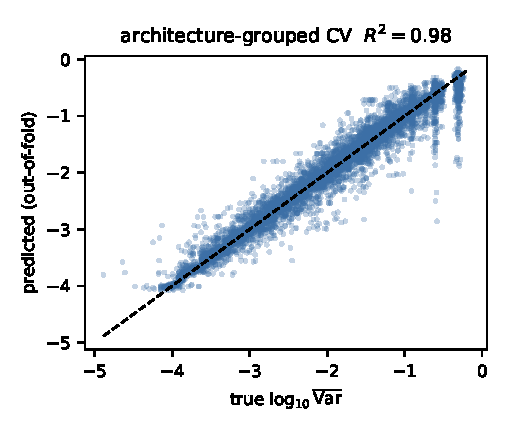
\includegraphics[width=0.58\textwidth]{figs/predicted.pdf}
\caption{Out-of-fold predicted versus true $\log_{10}\Vbar$ for the HGB
regressor under architecture-grouped cross-validation (first repeat). Every
point is predicted by a model that never saw its architecture. The dashed
line is $y=x$.}
\label{fig:predicted}
\end{figure}

\subsection{Extrapolation across qubit count}\label{sec:extrap}
Supplementary Tables~S4 and S6
report the qubit-count split, with
\ExtrapTrainRows{} training circuits at $n\le\ExtrapCut$ and
\ExtrapTestRows{} test circuits at $n\in\{11,12\}$. HGB attains
$R^2=\RsqExtrap$ (95\% CI $[\RsqExtrapLo,\RsqExtrapHi]$; seed spread
$\pm\RsqExtrapSeedSd$) and MAE \MaeExtrap{} (95\% CI
$[\MaeExtrapLo,\MaeExtrapHi]$). The five-coefficient physics-informed model reaches only
$R^2=\RsqExtrapPhys$: a single linear-in-$n$ slope per cost type, fitted on
$n\le\ExtrapCut$, does not describe the $n=11,12$ circuits. Two models do
well. The MLP reaches $R^2=\RsqExtrapMLPmean\pm\RsqExtrapMLPsd$ (mean and
standard deviation over ten random seeds), and the structured linear model
reaches \RsqExtrapStruct. Both are well above every tree ensemble, as
expected: a tree ensemble's prediction is constant outside the training
range of a feature, so it cannot continue the decay in $n$ past $n=10$,
whereas a model with continuous dependence on $n$ can. In-family the model
classes are equivalent; out of range the inductive bias decides.

Supplementary Table~S6 breaks the result down by qubit count and cost
locality. Error grows from $n=11$ to $n=12$ for both models, and global-cost
circuits at $n=12$ are the hardest subset (HGB $R^2=\RsqENOneTwoglobal$, MLP
\RsqEMNOneTwoglobal), as expected, since they are furthest from training in
both $n$ and label value. Every subset is predicted far better than the
subgroup-mean and physics-informed controls. The result should still be read
narrowly: in this split the test circuits are only two qubits beyond
training. This is not evidence of
unbounded extrapolation, and Section~\ref{sec:discussion} lists it as a
limitation.

Moving the training cutoff down (train on $n\le k$, test on all larger
circuits, $k=6,\dots,10$; Supplementary Figure~S8 and Table~S5) separates
the model classes further. At $k=6$ HGB falls to \GapHGBkSix, the structured
linear model holds at \GapStructkSix, and the MLP gives
$\GapMLPmeankSix\pm\GapMLPsdkSix$ over ten seeds, between \GapMLPminkSix{}
and \GapMLPmaxkSix. Section~\ref{sec:clifford} measures the same effect
with exact labels at larger sizes.


\paragraph{Beyond the training range: 13 and 14 qubits.} As a final
extrapolation test we generated a separate set of \LargeN{} circuits with
$n\in\{13,14\}$, labeled exactly as the main dataset, and scored models
trained on the full $n\le12$ dataset on it (Table~\ref{tab:large}, Supplementary Figure~S4).
The MLP reaches $R^2=\LargeRsqMLPmean\pm\LargeRsqMLPsd$ over ten seeds
(\LargeRsqMLPThirteen{} at $n=13$ and \LargeRsqMLPFourteen{} at $n=14$ for
the first seed), the structured linear model \LargeRsqStruct, HGB
\LargeRsqHGB, and the five-coefficient control \LargeRsqPhys. These circuits
are two to four times more expensive to label by statevector simulation
than the largest training circuits.

\begin{tableorg}[t]
\centering\tablebodyfont
\caption{Held-out 13- and 14-qubit circuits (\LargeN{} circuits, labeled as
the main dataset), predicted by models trained on all $n\le12$ circuits.
95\% bootstrap confidence intervals over test rows. Supplementary Table~S10
lists all models.}
\label{tab:large}
%%BEGIN-TABLE:large_short
\fittable{%
\begin{tabular}{lcccccc}
\toprule
Model & $R^2$ [95\% CI] & MAE & $R^2$, $n=13$ & $R^2$, $n=14$ & $R^2$, local & $R^2$, global \\
\midrule
MLP & 0.970 [0.965, 0.974] & 0.137 & 0.970 & 0.969 & 0.971 & 0.943 \\
Structured linear & 0.951 [0.945, 0.956] & 0.183 & 0.950 & 0.952 & 0.947 & 0.919 \\
Hist Gradient Boosting & 0.905 [0.898, 0.913] & 0.316 & 0.939 & 0.876 & 0.942 & 0.749 \\
Physics-informed linear & 0.350 [0.326, 0.375] & 0.815 & 0.354 & 0.345 & 0.187 & 0.157 \\
\botrule
\end{tabular}%
}
%%END-TABLE:large_short
\end{tableorg}





\subsection{The prediction horizon, measured with exact labels up to 32 qubits}\label{sec:clifford}
How far beyond its training range can a predictor be trusted? The
Clifford-labeled circuits, which run from 2 to \ClQmax{} qubits, let us
measure this directly. For a model trained on circuits with $n\le k$ we
compute the mean absolute error at each distance $d=n_{\rm test}-k$ beyond
the training range and define the \emph{prediction horizon} $H(\varepsilon)$
as the largest $d$ up to which that error stays at or below $\varepsilon$.
We use $\varepsilon=0.3$, which means that predictions are within a factor
of two of the true variance on average, and $\varepsilon=0.5$, a factor of
three on average, and vary $k$ from 8 to 24. A 90\% interval for the
horizon comes from a bootstrap over the test circuits at each distance. The
neural network is used as an ensemble of \HzEnsemble{} networks that differ
only in their random seed; averaging removes the seed dependence noted in
Section~\ref{sec:extrap}. Because censoring removes most global-cost
circuits at large $n$, we report the horizon separately for local-cost
circuits, of which more than four fifths are resolved at every size, and
for all resolved circuits.

Figure~\ref{fig:horizon} and Table~\ref{tab:horizon} give the result. For
local-cost circuits and training ranges of 12, 16 and 20 qubits the
ensemble has $H(0.3)=\HzLocMLPkTwelve$, \HzLocMLPkSixteen{} and
\HzLocMLPkTwenty{} qubits (90\% intervals \HzLocMLPIntkTwelve,
\HzLocMLPIntkSixteen{} and \HzLocMLPIntkTwenty): the predictable range is
the training range plus five to six qubits. The horizon is shorter for the
smallest training range, \HzLocMLPkEight{} qubits for $k=8$ (interval
\HzLocMLPIntkEight): it grows with the training range before it levels
off. The values for all resolved
circuits are similar (\HzMLPkTwelve, \HzMLPkSixteen, \HzMLPkTwenty), but only
the first is free of survivorship: within six qubits of the training range,
\HzResGlobkTwelve\% of global-cost circuits are resolved for $k=12$, against
\HzResGlobkSixteen\% and \HzResGlobkTwenty\% for $k=16$ and $k=20$. The error grows steadily with distance; for local costs and $k=12$ it is
\HzMaeTwelveDOne{} one qubit beyond training, \HzMaeTwelveDFour{} at four
and \HzMaeTwelveDSix{} at six, just above the tolerance, and it keeps
growing beyond the horizon without a sharp transition. The
structured linear model is less accurate close to the training range, so
its horizon at $\varepsilon=0.3$ is shorter (\HzLocTablekTwelve{} qubits for
$k=12$, interval \HzLocTableIntkTwelve), but its error grows more slowly far
out. Its intervals are wide (for local costs, \HzLocTableIntkSixteen{} at
$k=16$ and \HzLocTableIntkTwenty{} at $k=20$) because its error stays close
to the tolerance over several qubits, which is a property of any threshold
metric and the reason we report intervals. At those training ranges the
horizons of the two models cannot be ranked. HGB, whose prediction is constant beyond the
training range, has a horizon of one to three qubits unless the training
range already covers the labels that occur at larger $n$.

\begin{tableorg}[t]
\centering\tablebodyfont
\caption{Prediction horizon $H(0.3)$ in qubits beyond the training range
$n\le k$: the largest distance up to which the mean absolute error on
resolved Clifford-labeled circuits stays at or below $0.3$ $\log_{10}$
units, with 90\% bootstrap intervals, for local-cost circuits and for all
resolved circuits. ``Resolved'' is the fraction of test circuits within six
qubits of the training range that are above the sampling resolution.
``$\ge$'' marks a horizon that reaches the largest circuits available
($n=\ClQmax$).}
\label{tab:horizon}
%%BEGIN-TABLE:horizon
\fittable{%
\begin{tabular}{rrcccccc}
\toprule
 & & \multicolumn{2}{c}{Resolved within $d\le6$} & \multicolumn{2}{c}{MLP ensemble, $H(0.3)$} & \multicolumn{2}{c}{Structured linear, $H(0.3)$} \\
\cmidrule(lr){3-4}\cmidrule(lr){5-6}\cmidrule(lr){7-8}
Train $n\le k$ & Circuits & local & global & local cost & all resolved & local cost & all resolved \\
\midrule
$k=8$ & 5032 & 99\% & 100\% & $3$ [3, 4] & $4$ [3, 4] & $4$ [4, 4] & $5$ [4, 5] \\
$k=12$ & 7941 & 99\% & 99\% & $5$ [5, 6] & $6$ [5, 6] & $4$ [3, 5] & $4$ [4, 4] \\
$k=16$ & 9115 & 95\% & 81\% & $6$ [4, 7] & $6$ [5, 6] & $3$ [2, 5] & $3$ [3, 5] \\
$k=20$ & 10266 & 84\% & 36\% & $6$ [6, 7] & $6$ [6, 6] & $6$ [3, 8] & $3$ [3, 6] \\
$k=24$ & 11026 & 81\% & 24\% & $\ge8$ [8, 8] & $\ge8$ [7, 8] & $\ge8$ [8, 8] & $\ge8$ [3, 8] \\
\botrule
\end{tabular}%
}
%%END-TABLE:horizon
\end{tableorg}

\begin{figure}[t]
\centering
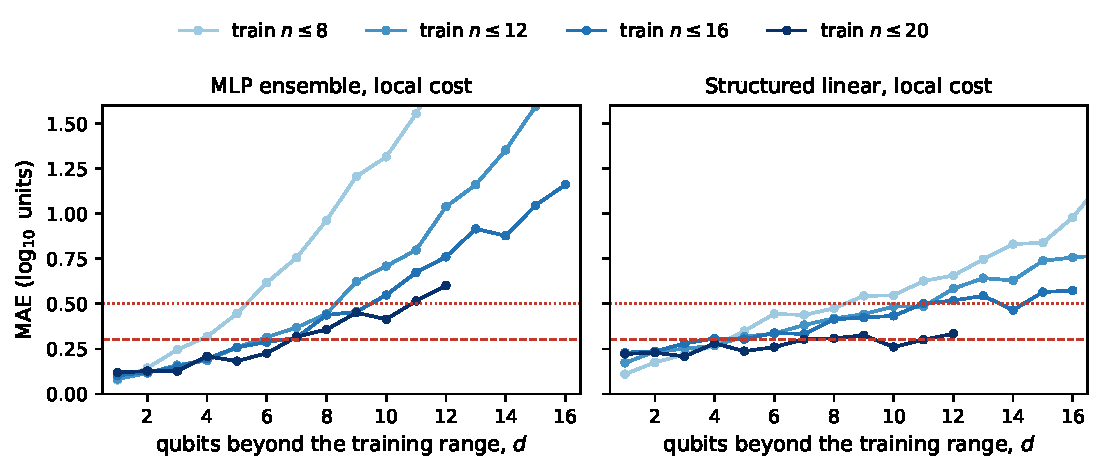
\includegraphics[width=\textwidth]{figs/horizon.pdf}
\caption{Mean absolute error on local-cost circuits against distance beyond
the training range, for four training ranges. Dashed and dotted lines mark the tolerances
$\varepsilon=0.3$ and $0.5$ that define the prediction horizon.}
\label{fig:horizon}
\end{figure}

\paragraph{Why there is a horizon.} Table~\ref{tab:clifford} (Supplementary
Figure~S7 and Table~S7) breaks the $k=12$ case down by cost locality, which
is necessary because censoring differs sharply between the two: of the
\ClCensored{} test circuits below the sampling resolution almost all have a
global cost, and beyond 24 qubits only about a quarter of global-cost
circuits are resolved, against more than four fifths of local-cost ones. An
$R^2$ computed on the resolved global-cost circuits at those sizes would
measure which circuits survive, not how well the model predicts, so we do
not report it.

%%CHECK-CL
\paragraph{Local costs: a genuine horizon.} For local costs the structured
linear model reaches $R^2=\ClLocStructA$ on 13--16 qubits and \ClLocStructB{}
on 17--20 qubits, then \ClLocStructC{} at
21--24, \ClLocStructD{} at 25--28 and \ClLocStructE{} at 29--32, with a bias
that grows steadily from $\ClLocBiasA$ to $\ClLocBiasE$. The neural network
matches it up to 20 qubits and then becomes seed-dependent and worse. The
cause is visible in the shallowest circuits. For local costs with $L\le3$
the true mean label is flat, $\ClShallowTrueA$ at 13--16 qubits and
$\ClShallowTrueE$ at 29--32, because the causal cone stops growing and
additional qubits change nothing that the observable can see. The model
predicts $\ClShallowStructA$ and $\ClShallowStructE$: it continues, more
weakly, the decay in qubit count that it learned below twelve qubits. The
cone features reduce this error but do not remove it, since below twelve
qubits the cone is rarely much smaller than the circuit and the model has
few examples of saturation to learn from.

\paragraph{Global costs: accurate where measurable.} For global costs the
structured model reaches $R^2=\ClGloStructA$ and \ClGloStructB{} at 13--16
and 17--20 qubits, with negligible bias. Beyond that most circuits are
censored and the only available test is whether a prediction respects the
measured upper bound on the label. At 21--24, 25--28 and 29--32 qubits,
\ClGloCensC\%, \ClGloCensD\% and \ClGloCensE\% of the predictions for
censored circuits do. Even at 17--20 qubits, where few global-cost
circuits are censored, only \ClGloCensB\% of the predictions for those few
respect the bound. Just beyond the resolution limit the model therefore
predicts a variance that is too large: it rates the flattest circuits as
less flat than they are, which is the costly direction for a screening
tool, and the accuracy quoted above holds for resolved circuits only. At
the largest sizes the predictions are consistent with the bound. Tree ensembles predict a constant outside their
training range; their apparent scores on the resolved circuits at large $n$
(Supplementary Table~S7) reflect the same survivorship and should not be
read as extrapolation.

\paragraph{Extending the horizon, and an open problem.} The horizon moves
with the training range. When the training range is extended to $n\le20$
with Clifford labels, the same models predict the resolved 21- to 32-qubit
circuits with $R^2=\ClLeTwentyStruct$ (structured linear),
$\ClLeTwentyMLP$ (neural network, five seeds) and \ClLeTwentyHGB{} (HGB),
computed on the \ClLeTwentyResolved{} resolved circuits of the
\ClLeTwentyTotal{} with $n>20$. That HGB scores highest shows what this
number measures: the resolved large-$n$ circuits then lie within the range
of labels seen in training, so the task has become interpolation in label,
and the censored circuits are not tested.

Predicting reliably beyond five to six qubits from a training range of 12
or more qubits is
therefore open, and within the horizon the statement holds for circuits
whose variance can be resolved. Two ingredients are missing. One is a model whose
dependence on qubit count saturates with the causal cone instead of
continuing a decay, which would remove the bias for local costs. The other
is a label for the flattest circuits, which sampling cannot resolve and
for which the present models err in the costly direction. The released
circuits with exact labels up to \ClQmax{} qubits, together with the metric
$H(\varepsilon)$, define a benchmark for this problem: a method that
extends $H(0.3)$ beyond six qubits from a 12-qubit training range, on the
same circuits, would be a clear improvement.

\begin{tableorg}[t]
\centering\tablebodyfont
\caption{Extrapolation with exact Clifford labels, by cost locality. Models
are trained on $n\le12$ (\ClTrainRows{} circuits). ``Resolved'' is the
fraction of test circuits above the sampling resolution; $R^2$ and bias
(mean prediction minus mean label, structured linear model) are computed on
resolved circuits and are omitted where fewer than half are resolved.
``Censored OK'' is the fraction of censored circuits whose prediction
respects the measured upper bound. MLP: mean $\pm$ standard deviation over
ten seeds.}
\label{tab:clifford}
%%BEGIN-TABLE:clifford_cost
\fittable{%
\begin{tabular}{lcccccccc}
\toprule
 & \multicolumn{4}{c}{Local cost} & \multicolumn{4}{c}{Global cost} \\
\cmidrule(lr){2-5}\cmidrule(lr){6-9}
Qubits & Resolved & Struct.~$R^2$ & MLP $R^2$ & Bias & Resolved & Struct.~$R^2$ & Bias & Censored OK \\
\midrule
13--16 & 98\% & 0.92 & $0.96 \pm 0.01$ & $-0.14$ & 100\% & 0.87 & $-0.01$ & -- \\
17--20 & 97\% & 0.89 & $0.87 \pm 0.05$ & $-0.23$ & 94\% & 0.84 & $-0.07$ & 5\% \\
21--24 & 86\% & 0.78 & $0.39 \pm 0.27$ & $-0.40$ & 41\% & -- & -- & 35\% \\
25--28 & 82\% & 0.43 & $-1.51 \pm 1.29$ & $-0.66$ & 25\% & -- & -- & 60\% \\
29--32 & 81\% & 0.23 & $-4.04 \pm 2.70$ & $-0.77$ & 22\% & -- & -- & 98\% \\
\botrule
\end{tabular}%
}
%%END-TABLE:clifford_cost
\end{tableorg}


\subsection{What drives trainability}\label{sec:ablation}
Table~\ref{tab:ablation} reports the feature ablation, in two parts. The first part asks what the derived features add
to the six design parameters. In-family they add almost nothing: the six
primitive features alone reach $R^2=\RsqPrim$, and adding the effective
weight, the causal cone, or all derived features changes this by
\DeltaAddBoth{} or less. A tree ensemble reconstructs these quantities from
the primitives when it has seen every architecture's neighbors. Their value
appears out of range: they raise transfer to unseen entanglement patterns
(Section~\ref{sec:lopo}) and extrapolation in qubit count
(Sections~\ref{sec:extrap} and \ref{sec:clifford}), where the model must
rely on structure it cannot interpolate.

The second part removes one primitive feature at a time from the
six-feature model. Two cautions apply to its reading. The drop measures
information that the remaining features cannot supply, so a feature that is
implied by the others scores low however relevant it is. And a large drop
does not mean that the variable explains the label on its own; the
cost-locality subgroup mean of Table~\ref{tab:models} scores only
$R^2=\RsqSub$. Most of the information enters through interactions. With
that understood, the largest drops come from \AblTopOne{}
($\Delta R^2=\AblTopOneDelta$), \AblTopTwo{} (\AblTopTwoDelta), and
\AblTopThree{} (\AblTopThreeDelta). The entangler gate costs
\DeltaGatePrim{} even though the mean labels of CZ and CX circuits differ by
only \GateGap. Table~\ref{tab:effweight} resolves this
apparent contradiction. The entangler gate matters mainly because it
decides what is measured. With CX, the nominally local cost on a circular
pattern has effective weight $n-1$ and the lowest mean label of all
local-cost families, and the nominally global cost on an all-to-all pattern
has effective weight $1$ and the highest mean label of all global-cost
families. The label tracks the effective weight, not the nominal one. This
is the cost-locality effect of Cerezo et al.~\cite{cerezo2021cost} applied
to the observable that is actually measured, and it is why the
five-coefficient model improves from \RsqPhys{} to \RsqPhysEff{} when the
nominal indicator is replaced by the effective weight. The ablation is a
consistency check on the model, not an independent discovery: the features
were chosen with the theory in mind.

\begin{tableorg}[t]
\centering\tablebodyfont
\caption{Nominal and effective observable weight for circuits with
$n\ge10$, with the mean label of each family. CZ leaves the observable
unchanged; CX maps it to a different $Z$-string.}
\label{tab:effweight}
%%BEGIN-TABLE:effweight
\fittable{%
\begin{tabular}{lllcrr}
\toprule
Gate & Pattern & Nominal cost & Effective weight & Mean $\log_{10}\overline{\mathrm{Var}}$ & Circuits \\
\midrule
CZ & linear & local & $1$ & $-1.25$ & 491 \\
CZ & linear & global & $n$ & $-3.37$ & 481 \\
CZ & circular & local & $1$ & $-1.81$ & 425 \\
CZ & circular & global & $n$ & $-3.42$ & 503 \\
CZ & all-to-all & local & $1$ & $-2.67$ & 416 \\
CZ & all-to-all & global & $n$ & $-3.14$ & 471 \\
\midrule
CX & linear & local & $1$ & $-2.07$ & 435 \\
CX & linear & global & $\approx n/2$ & $-3.22$ & 410 \\
CX & circular & local & $n-1$ & $-3.32$ & 467 \\
CX & circular & global & $\approx n/2$ & $-3.26$ & 413 \\
CX & all-to-all & local & $1$ & $-2.70$ & 455 \\
CX & all-to-all & global & $1$ & $-2.13$ & 443 \\
\botrule
\end{tabular}%
}
%%END-TABLE:effweight
\end{tableorg}

\begin{tableorg}[t]
\centering\tablebodyfont
\caption{Feature ablation under architecture-grouped cross-validation
(HGB; mean $\pm$ standard deviation over \NFolds{} folds). Upper part:
what the derived features add to the six primitive features. Lower part:
the drop when one primitive feature is removed from the six.}
\label{tab:ablation}
%%BEGIN-TABLE:ablation
\fittable{%
\begin{tabular}{lcc}
\toprule
Feature set & $R^2$ (grouped CV) & $\Delta R^2$ \\
\midrule
six primitive features & $0.980 \pm 0.003$ & -- \\
\quad + effective weight & $0.981 \pm 0.003$ & $0.002 \pm 0.001$ \\
\quad + causal cone & $0.981 \pm 0.003$ & $0.001 \pm 0.001$ \\
\quad + effective weight + causal cone & $0.981 \pm 0.003$ & $0.001 \pm 0.001$ \\
all 12 features & $0.980 \pm 0.003$ & $0.000 \pm 0.001$ \\
\midrule
primitive minus qubit count $n$ & $0.259 \pm 0.021$ & $0.721 \pm 0.019$ \\
primitive minus layers $L$ & $0.721 \pm 0.022$ & $0.259 \pm 0.021$ \\
primitive minus rotation scheme & $0.938 \pm 0.005$ & $0.042 \pm 0.003$ \\
primitive minus entanglement pattern & $0.795 \pm 0.020$ & $0.184 \pm 0.019$ \\
primitive minus entangler gate & $0.825 \pm 0.017$ & $0.155 \pm 0.018$ \\
primitive minus cost locality & $0.676 \pm 0.028$ & $0.304 \pm 0.027$ \\
\botrule
\end{tabular}%
}
%%END-TABLE:ablation
\end{tableorg}


\subsection{Transfer to unseen entanglement patterns}\label{sec:lopo}
Table~\ref{tab:lopo} (Supplementary Figure~S6) reports the leave-one-pattern-out
experiment. With the graph descriptors in place of the pattern index, the
pooled five-pattern model loses nothing in-family (grouped-CV
$R^2=\LopoDescRsq$ with descriptors versus \LopoIndexRsq{} with the index).
When a pattern is held out entirely, the outcome depends on two things:
whether the model is given the physics features, and where the pattern's
descriptors fall relative to the training patterns. With graph descriptors
alone (Table~\ref{tab:lopo}, third column) transfer is partial: brickwork,
whose union graph is the same chain as linear and whose descriptors lie
inside the training range, reaches $R^2=\LopoBrickNoPhys$, but linear
(\LopoLinearNoPhys), circular (\LopoCircularNoPhys) and star
(\LopoStarNoPhys) are predicted only moderately and all-to-all, the extreme
of every descriptor, fails (\LopoAllNoPhys). Adding the effective observable
weight and the causal cone changes the picture. These two quantities are
computed for the held-out pattern from its own gate list, so the model
receives, in closed form, the part of the pattern's effect that acts through
the observable. Held-out linear is then predicted with $R^2=\LopoLinearUnseen$
(\LopoLinearSeen{} when seen), circular with \LopoCircularUnseen{}
(\LopoCircularSeen), brickwork with \LopoBrickUnseen{} (\LopoBrickSeen), star
with \LopoStarUnseen{} (\LopoStarSeen), and even all-to-all with
\LopoAllUnseen{} (\LopoAllSeen), far above the physics-informed control
(\LopoAllPhys). The classifier is more forgiving still: AUC is at least
\LopoMinAuc{} for every held-out pattern.

Two readings follow. First, transfer to a pattern the model has never seen
is possible when the pattern is described by what it does to the observable
and to the causal cone, rather than by a name. Second, it is not free:
every held-out pattern is still predicted worse than a seen one, and the
extreme pattern loses the most. A user who needs the best accuracy for a new
gate pattern should add a modest number of labeled circuits of that pattern
to the training set, which the released pipeline does from one command.

\begin{tableorg}[t]
\centering\tablebodyfont
\caption{Leave-one-pattern-out transfer. For each row, HGB is trained on the
other four patterns and tested on the held-out one (``unseen''), with the
full pattern-agnostic feature set or with graph descriptors only (``graph
only'', no effective weight and no causal cone); ``seen'' scores the same
rows under architecture-grouped cross-validation on the pooled data; the
physics-informed linear control (effective-weight variant) is fitted on the
same training rows.}
\label{tab:lopo}
%%BEGIN-TABLE:lopo
\fittable{%
\begin{tabular}{lrccccccc}
\toprule
 & & \multicolumn{3}{c}{Pattern unseen} & \multicolumn{2}{c}{Pattern seen} & \multicolumn{2}{c}{Physics-linear} \\
\cmidrule(lr){3-5}\cmidrule(lr){6-7}\cmidrule(lr){8-9}
Held-out pattern & Rows & $R^2$ & $R^2$, graph only & MAE & $R^2$ & MAE & $R^2$ & MAE \\
\midrule
linear & 6608 & 0.946 & 0.732 & 0.128 & 0.983 & 0.068 & 0.692 & 0.400 \\
circular & 6709 & 0.950 & 0.694 & 0.132 & 0.985 & 0.058 & 0.824 & 0.310 \\
all-to-all & 6541 & 0.753 & 0.414 & 0.241 & 0.972 & 0.076 & 0.621 & 0.442 \\
brickwork & 4998 & 0.930 & 0.925 & 0.141 & 0.978 & 0.074 & 0.669 & 0.409 \\
star & 4928 & 0.924 & 0.742 & 0.156 & 0.968 & 0.083 & 0.726 & 0.391 \\
\botrule
\end{tabular}%
}
%%END-TABLE:lopo
\end{tableorg}


\subsection{Other circuit families}\label{sec:families}
Table~\ref{tab:families} repeats the central measurements on the two further
families of Section~\ref{sec:familiesmethod}. The picture is the same in all
three. On unseen architectures the learners reach $R^2=\TiedHGB$ and
\TiedMLP{} for shared parameters and \GraphHGB{} and \GraphMLP{} for random
graphs, against \RsqCV{} and \RsqCVMLP{} for the named patterns, and in
each family a fitted linear rule comes within a few hundredths
(\TiedRule{} and \GraphRule). Extrapolation from $n\le10$ to 11 and 12
qubits also behaves alike: the neural network and the linear rule continue
the trend, and tree ensembles do so only where the labels at larger $n$
stay within the training range.

Three family-specific observations are worth recording. First, shared
parameters change the label substantially. A model trained on the
independent-parameter family and applied to the shared-parameter family
fails ($R^2=\TiedTransfer$): on identical architectures the shared-parameter
label is higher by \TiedOffset{} $\log_{10}$ units on average, because the
gradient of a shared angle sums the contributions of $n$ gates, and the two
labels correlate only at \TiedCorr. A predictor must be fitted per family.
Second, the shared-parameter
family is one to which the Clifford shortcut does not apply
(Section~\ref{sec:familiesmethod}). Trained on $n\le12$, the models predict
the held-out 13- and 14-qubit shared-parameter circuits with
$R^2=\TiedLargeMLP$ (neural network, ten seeds), \TiedLargeRule{} (linear
rule) and \TiedLargeHGB{} (HGB); \TiedLargeBelowCut\% of these circuits lie
below the cutoff. HGB scores above the linear rule here only because
\TiedLargeInRange\% of the labels at these sizes lie within the range seen
in training, so that little extrapolation of the label is needed; this is
the same condition under which it does well in
Section~\ref{sec:clifford}, and does not contradict its failure to
extrapolate. We note that this family is not strongly
flat at these sizes, so the test shows that the approach carries over, not
that it resolves deep plateaus where no exact label exists. Third, on random graphs the physics
descriptors are what make the problem tractable. HGB given only the seven
design parameters reaches $R^2=\GraphDesignOnly$; given the descriptors it
reaches \GraphHGB. The causal-cone fraction equals the exact non-structural
fraction of parameters in \GraphConeExactRy\% of fixed-\texttt{ry} random-graph
circuits (mean absolute difference \GraphConeMadRy), although no two
circuits share a graph.

\begin{tableorg}[t]
\centering\tablebodyfont
\caption{The central measurements on three circuit families. ``Fitted
linear rule'' is the structured linear model for the first two families and
its descriptor analogue for random graphs. Unseen architectures: grouped
cross-validation for the first two families, repeated five-fold
cross-validation for random graphs, where every circuit is a distinct
architecture (mean $\pm$ standard deviation over ten folds).}
\label{tab:families}
%%BEGIN-TABLE:families
\fittable{%
\begin{tabular}{lccc}
\toprule
 & Named patterns & Shared parameters & Random graphs \\
\midrule
Circuits & 19858 & 9929 & 9949 \\
Exact Clifford shortcut & yes & no & yes \\
Noise ceiling on $R^2$ & 0.985 & 0.989 & -- \\
\midrule
\multicolumn{4}{l}{\emph{Unseen architectures, $R^2$}}\\
\quad HGB & $0.980 \pm 0.003$ & $0.983 \pm 0.002$ & $0.975 \pm 0.002$ \\
\quad MLP & $0.979 \pm 0.003$ & $0.981 \pm 0.002$ & $0.974 \pm 0.002$ \\
\quad fitted linear rule & $0.969 \pm 0.002$ & $0.958 \pm 0.005$ & $0.966 \pm 0.003$ \\
\quad five-coefficient rule & $0.682 \pm 0.016$ & $0.309 \pm 0.039$ & -- \\
\midrule
\multicolumn{4}{l}{\emph{Trained on $n\le10$, tested on $n=11,12$, $R^2$}}\\
\quad MLP (10 seeds) & $0.961 \pm 0.003$ & $0.969 \pm 0.003$ & $0.923 \pm 0.006$ \\
\quad HGB & 0.860 & 0.942 & 0.684 \\
\quad fitted linear rule & 0.935 & 0.934 & 0.902 \\
\midrule
\multicolumn{4}{l}{\emph{Trained on $n\le12$, tested on $n=13,14$, $R^2$}}\\
\quad MLP (10 seeds) & $0.972 \pm 0.002$ & $0.980 \pm 0.001$ & -- \\
\quad HGB & 0.905 & 0.960 & -- \\
\quad fitted linear rule & 0.951 & 0.940 & -- \\
\botrule
\end{tabular}%
}
%%END-TABLE:families
\end{tableorg}

\subsection{Ranking circuits at fixed qubit count}\label{sec:screening}
The intended use of the predictor is to rank candidate architectures and
pass the most promising ones to a more expensive evaluation. A global
ranking is not an informative test of this use. Every circuit in the dataset
with $n\le\AllAboveMaxN$ lies above the cutoff, as do all but \BelowAtFive{}
of the \RowsAtFive{} circuits with $n=5$, so ranking by qubit count alone
selects
a top fifth that is entirely above the cutoff (\ScreenByNPrec\% precision,
\ScreenByNRecall\% recall), and the predictor does the same. The informative
question is whether the predictor ranks circuits correctly \emph{within} a
fixed qubit count, where size carries no information.
Table~\ref{tab:screening} answers it with out-of-fold predictions from a
five-fold architecture-grouped split (a separate fold assignment from the
one used in Section~\ref{sec:cv}). For every $n$ at which both classes occur, the rank
correlation between the HGB prediction and the true label lies between
\ScrSpHGBmin{} and \ScrSpHGBmax, against \ScrSpPhysmin{} to \ScrSpPhysmax{}
for the five-coefficient model; the structured linear model is again close
to HGB (\ScrSpStructmin{} to \ScrSpStructmax). At $n=12$, where only
\ScrAboveTwelve\% of circuits are above the cutoff, \ScrPrecTwelve\% of the
top fifth of the HGB ranking are. The top fifth is a shortlist, not a
complete list: by construction it contains at most a fifth of the circuits
and so misses the remaining ones above the cutoff.

\begin{tableorg}[t]
\centering\tablebodyfont
\caption{Ranking within a fixed qubit count, from out-of-fold predictions.
Spearman correlation between predicted and true label, and the percentage
of the top 20\% of each ranking that lies above the cutoff $y\ge-2$. Qubit
counts at which every circuit is above the cutoff are omitted.}
\label{tab:screening}
%%BEGIN-TABLE:screening_within
\fittable{%
\begin{tabular}{rrccccccc}
\toprule
 & & & \multicolumn{3}{c}{Spearman $\rho$ with true label} & \multicolumn{3}{c}{Above cutoff in top 20\% (\%)} \\
\cmidrule(lr){4-6}\cmidrule(lr){7-9}
$n$ & Circuits & Above cutoff (\%) & HGB & Struct.~linear & Physics-linear & HGB & Struct.~linear & Physics-linear \\
\midrule
5 & 1745 & 100 & 0.937 & 0.916 & 0.578 & 100.0 & 100.0 & 100.0 \\
6 & 1778 & 69 & 0.943 & 0.912 & 0.640 & 99.7 & 100.0 & 94.9 \\
7 & 1755 & 38 & 0.959 & 0.934 & 0.619 & 99.7 & 99.7 & 83.2 \\
8 & 1901 & 27 & 0.968 & 0.946 & 0.622 & 99.2 & 98.9 & 68.9 \\
9 & 1876 & 26 & 0.970 & 0.958 & 0.632 & 98.9 & 98.9 & 70.7 \\
10 & 1830 & 25 & 0.971 & 0.958 & 0.623 & 100.0 & 99.7 & 66.9 \\
11 & 1740 & 24 & 0.977 & 0.964 & 0.610 & 99.7 & 99.4 & 67.0 \\
12 & 1840 & 26 & 0.978 & 0.968 & 0.605 & 99.5 & 99.7 & 64.9 \\
\botrule
\end{tabular}%
}
%%END-TABLE:screening_within
\end{tableorg}

%=================================================================
\section{Discussion}\label{sec:discussion}

Our results support one main claim, stated within its scope. For the
hardware-efficient family studied here, the mean gradient variance is a
simple function of the architecture. Within each combination of categorical
design choices it falls linearly in $\log_{10}$ with qubit count and
saturates with depth, and a model of that form, or a flexible learner that
knows nothing of the form, predicts it close to the noise ceiling of the label for
architectures it has never seen. The effective weight of the measured observable lifts the
five-coefficient rule from \RsqPhys{} to \RsqPhysEff, and together with the
causal cone it is what lets predictions transfer outside the training
range; within it, a flexible learner reconstructs both.

In practice the predictor can rank a large space of candidate ans\"atze at
microseconds per candidate, for example as a zero-cost filter inside a QAS
loop, leaving expensive estimation for a shortlist
(Section~\ref{sec:screening}).

Several limitations scope these claims.
(i)~\emph{Hardware-efficient circuits only.} The design spaces studied are
variants of one hardware-efficient layout: five named entanglement patterns,
random entangling graphs, and independent or layer-shared parameters. Section~\ref{sec:lopo} shows
that a pattern the model has never seen can be predicted when it is
described by its effect on the observable and on the causal cone, but with
a measurable loss, so predictions for a new gate pattern should be
supported by some labeled circuits of that pattern. The pipeline generates
them from one command. Predictions outside the hardware-efficient family
(for example, problem-inspired ans\"atze with their own gate sets) are
unsupported.
(ii)~\emph{Finite size.} Statevector labels exist only at $n\le14$.
Clifford labels reach any $n$ but resolve only variances above
$100/(2^{20}nL)$, between about $10^{\ClFloorMinExp}$ and
$10^{\ClFloorMaxExp}$ depending on the number of parameters. A barren
plateau is a statement about scaling as $n\to\infty$; our label is a
finite-size proxy, and the extrapolation results cover two additional
qubits with statevector labels and five to six with Clifford labels (from training ranges of 12 or more
qubits; three from a range of 8), for
resolved circuits, not an asymptotic regime. For the flattest global-cost
circuits just beyond the sampling resolution the models overestimate the
variance, the costly direction for screening. Tree ensembles cannot continue a trend in $n$ beyond
the training range, and the neural network is seed-dependent at large
gaps, so a user who needs predictions at larger $n$ should prefer the
structured model, or extend the training range with Clifford labels.
(iii)~\emph{Ideal simulation.} We use a noiseless statevector simulator, so
noise-induced plateaus~\cite{wang2021noise} are out of scope.
(iv)~\emph{Label noise, hidden axes, and the cutoff.} Each variance is
estimated from \Samples{} samples (mean absolute relabeling difference
\RepeatMAD{} in $\log_{10}$ units); for random-Pauli circuits the drawn axis
pattern is not part of the feature vector, which we quantified as a noise
ceiling; and the barren cutoff $y<-2$ is a modeling choice that affects
only the classification results (Supplementary Table~S3).
(v)~\emph{Exact alternatives for this family.} Because every angle
appears once with a Pauli generator, the gradient variance of these
circuits can be estimated exactly by Clifford sampling at any qubit count
(Section~\ref{sec:clifford}), at a cost of seconds per circuit. This
weakens the argument that labels are expensive. Three things remain in
favor of a predictor: it costs microseconds per candidate, which matters
when the design space is searched; sampling cannot resolve variances far
below the reciprocal of the sample count, which is where barren plateaus
live; and the quadrature property fails as soon as parameters are shared
between gates or generators are not Paulis. The shared-parameter family of
Section~\ref{sec:families} is such a case: the Clifford shortcut does not
apply to it, and a fitted predictor is as accurate there as for the
independent-parameter family, at the sizes we could test.
(vi)~\emph{Gradient variance is not optimization outcome.} The label measures
how flat the landscape is on average, not whether training succeeds. As a
check we trained several hundred fresh circuits from the same design space
with gradient descent and with Adam, with exact gradients and with
gradients estimated from 100 or 1\,000 shots, for 200 steps from random
starts (four configurations, \TOCircuitsMin{} to \TOCircuitsMax{} circuits
each, three restarts per circuit; code and results are in the repository).
At $n\le12$ between \TOFracMin\% and \TOFracMax\% of circuits decreased the
cost by more than $0.5$ (of a possible range of $2$) regardless of their
label, and the rank correlation between the label and the loss decrease
was between \TORhoTrueMin{} and \TORhoTrueMax{} (\TORhoPredMin{} to
\TORhoPredMax{} for the predicted label). At these sizes even
the smallest labels in the dataset correspond to typical gradient
components between $10^{-3}$ and $10^{-2}$, which a modest shot budget resolves. The
predictor should therefore be read as a screen for the gradient-variance
scaling that becomes prohibitive at larger $n$, not as a forecast of
optimization success at the sizes simulated here.
(vii)~\emph{Averaging over parameters.} The mean over parameters of the
gradient variance is one summary of a circuit's landscape. Other summaries,
such as the minimum over parameters or the distribution across layers, may
matter for particular optimizers. We release all per-circuit statistics
(mean, median, minimum, maximum, and the structural-zero count) so these can
be studied.



%=================================================================
\section{Conclusion}\label{sec:conclusion}

We studied how well the gradient variance of hardware-efficient
variational circuits can be predicted from architecture alone. With the
label defined as the mean over all parameters and structural zeros removed,
the answer is: almost completely, and by a simple rule. Learners reach
$R^2\approx\RsqCV$ on unseen architectures against a noise ceiling of
\RsqCeiling, a structured linear model reaches \RsqStruct, and a
five-coefficient textbook rule \RsqPhys; the same holds for circuits with
layer-shared parameters, to which the Clifford shortcut does not apply, and
for random entangling graphs. Two closed-form quantities, the effective
weight of the observable and the causal cone, add little within the
training range but allow transfer to entanglement patterns absent from
training. With exact labels up to 32 qubits we measured a prediction
horizon: for local costs, five to six qubits beyond a training range of 12
or more qubits and three beyond a range of 8, on
average within a factor of two of the true variance. Beyond it, and for the
flattest global-cost circuits, the models err in the direction that
matters for screening, rating circuits as less flat than they are. Extending that horizon, and resolving the flattest circuits, are
open problems for which the released circuits and the horizon metric
provide a benchmark. Noisy circuits and ans\"atze outside the
hardware-efficient layout are natural next steps.

%=================================================================
\backmatter

\bmhead{Acknowledgements}
During the preparation of this manuscript, the author used ChatGPT (OpenAI)
and Claude (Anthropic) for language editing, grammar correction, and
refinement of the written text, and for assistance in developing the
accompanying open-source research code. The author reviewed and edited all
content and takes full responsibility for the content of the publication.

\section*{Declarations}

\begin{itemize}
\item \textbf{Funding.} This research received no external funding.
\item \textbf{Conflict of interest.} The author declares no competing interests.
\item \textbf{Ethics approval and consent to participate.} Not applicable.
\item \textbf{Consent for publication.} Not applicable.
\item \textbf{Data availability.} The dataset supporting this study is openly
available in Zenodo at \url{https://doi.org/10.5281/zenodo.21446194} and in the
repository at \url{https://github.com/bithabib/quantum_computer_simulator}. It
contains the full labeled dataset of \Nrows{} variational circuits, including
the per-circuit gradient-variance statistics, the datasets for the
unseen-pattern, 13--14-qubit, Clifford-sampling, shared-parameter and
random-graph experiments, and
regenerates from the sequence of commands documented in the repository,
with
fixed random seeds (root seed 12345 for data generation, seed 0 for all
models). Software: Python \PythonVersion, NumPy \NumpyVersion, scikit-learn
\SklearnVersion.
\item \textbf{Materials availability.} Not applicable.
\item \textbf{Code availability.} All code (the statevector simulator, the
adjoint-gradient routine, the dataset generator, the validation script, and
the analysis script that produces every table and figure in this article) is
openly available in the same repository.
\item \textbf{Author contribution.} M.H.R. is the sole author and is responsible
for all aspects of the work.
\end{itemize}

%=================================================================
\bibliography{refs}

\end{document}
